\PassOptionsToPackage{usenames,x11names,dvipsnames}{xcolor}
\documentclass[technote,10pt]{IEEEtran}
\usepackage[T1]{fontenc}
\usepackage{lmodern}
\usepackage{amsmath,amssymb,mathtools,bm}
\usepackage{booktabs,tabularx,array}
\usepackage{graphicx}
\usepackage{dblfloatfix}
\usepackage{microtype}
\usepackage{etoolbox}
\makeatletter
\patchcmd{\thebibliography}{\footnotesize\vskip}{\footnotesize\linespread{0.90}\selectfont\vskip}{}{}
\makeatother
\def\IEEEbibitemsep{-0.8pt}
\usepackage{tikz}
\usetikzlibrary{arrows.meta,positioning,calc,fit}
\usetikzlibrary{external}
% Cache externalized vector PDFs inside tex/Figures/External.
% Global opt-out; only selected figures are externalized.
\tikzexternalize[prefix=Figures/External/]
% Plain pdflatex: render inline, with no shell-escape requirement.
% pdflatex -shell-escape: create/reuse external vector PDFs.
\newif\ifDTAGExternalPDF
\ifnum\pdfshellescape=1
  \DTAGExternalPDFtrue
\else
  \DTAGExternalPDFfalse
\fi
\newcommand{\DTAGExternalEnable}{\ifDTAGExternalPDF\tikzexternalenable\fi}
\tikzexternaldisable
\usepackage{pgfplots}
\usepackage{pgfplotstable}
\pgfplotsset{compat=1.18}
\usepgfplotslibrary{groupplots,fillbetween}
\usepackage{cite}
\usepackage[hidelinks]{hyperref}
\newcommand{\EE}{\mathbb{E}}
\newcommand{\calS}{\mathcal{S}}
\newcommand{\calB}{\mathcal{B}}
\newcommand{\calX}{\mathcal{X}}
\newcommand{\JS}{D_{\mathrm{JS}}}
\newcommand{\Ph}{\Phi}
\newcommand{\Do}{\operatorname{do}}
\newcommand{\supp}{\operatorname{supp}}
\newcommand{\KL}{D_{\mathrm{KL}}}
\definecolor{dtred}{RGB}{133,39,48}
\definecolor{dtblue}{RGB}{34,68,116}
\definecolor{dtgray}{RGB}{120,120,124}
\definecolor{dtmint}{RGB}{224,245,240}
\definecolor{dtpale}{RGB}{225,237,251}
\definecolor{dtorange}{RGB}{247,231,207}
\pgfplotsset{
  publication axis/.style={
    axis line style={draw=black,line width=.85pt},
    tick style={draw=black,line width=.8pt},
    tick label style={font=\footnotesize\bfseries,text=black},
    label style={font=\small\bfseries,text=black},
    title style={font=\small\bfseries,text=black},
    grid=major,grid style={draw=black!12,line width=.25pt},
    scaled ticks=false
  }
}

\definecolor{modblue}{RGB}{24,70,120}
\definecolor{modred}{RGB}{162,62,67}
\definecolor{modteal}{RGB}{22,117,108}
\title{Digital Twin Anchored Generation: Adaptive Questioning for Directed Movement in Opinion Space}
\author{Ishanu Chattopadhyay%
\thanks{Email: ishanu\_ch@uky.edu Working research draft, October 2026. University of Kentucky. Native GSS 2024 computational experiments and human-response study.}}


% ###################################
\newcommand{\mnp}[2]{\begin{minipage}{#1}#2\end{minipage}} 
\newcommand{\xtitaut}[2]{
  \noindent\mnp{\textwidth}{
    \mnp{\textwidth}{\raggedright\Huge \bf \sffamily #1}

    \vskip 1em

    {\bf \sffamily #2}
  }
  \vskip 2em
}



\begin{document}
% Source data are external CSVs (not generated TeX files).
% The build script links tex/figures to the desired completed experiment.
% The stable path is required by external TikZ subprocesses.
\providecommand{\DTAGFigureDir}{Figures}
\def\DTAGMetadataCSV{\DTAGFigureDir/publication_metadata.csv}
\pgfplotstableread[col sep=comma]{\DTAGMetadataCSV}\DTAGMetadataTable
\pgfplotstablegetelem{0}{steps}\of{\DTAGMetadataTable}\xdef\DTAGSteps{\pgfplotsretval}
\pgfplotstablegetelem{0}{reps}\of{\DTAGMetadataTable}\xdef\DTAGReps{\pgfplotsretval}
\pgfplotstablegetelem{0}{displayed_questions}\of{\DTAGMetadataTable}\xdef\DTAGIdMax{\pgfplotsretval}
\pgfplotstablegetelem{0}{total_questions}\of{\DTAGMetadataTable}\xdef\DTAGTotalQuestions{\pgfplotsretval}
\pgfplotstablegetelem{0}{endpoint_bound}\of{\DTAGMetadataTable}\xdef\DTAGEndpointBound{\pgfplotsretval}
\pgfplotstablegetelem{0}{trajectory_bound}\of{\DTAGMetadataTable}\xdef\DTAGTrajectoryBound{\pgfplotsretval}
\pgfplotstablegetelem{0}{order_bound}\of{\DTAGMetadataTable}\xdef\DTAGOrderBound{\pgfplotsretval}
\pgfmathsetmacro{\DTAGXMax}{\DTAGSteps+0.5}
\pgfmathsetmacro{\DTAGYMax}{\DTAGReps+0.5}
\pgfmathtruncatemacro{\DTAGHalfSteps}{round(\DTAGSteps/2)}
\pgfmathtruncatemacro{\DTAGHalfReps}{round(\DTAGReps/2)}

%\xtitaut{\title}{Ishanu Chattopadhyay}
\maketitle


\begin{abstract}
Can the choice of survey questions steer inferred ideology without controlling the answers? Digital Twin Anchored Generation (DTAG) uses Large Science Model (LSM) conditionals to select questions maximizing expected displacement along a pole-relative ideology index. In 960 GSS 2024 twenty-question simulations across six personas, directional policies shifted the index as intended without asking any of the 27 pole-defining items; 2,880 fixed-set replays preserved direction under reordering. In a prospective Prolific human study (34 completed sessions), mean shifts were $-0.0783$ (Left) and $+0.0382$ (Right), with 95\% participant-bootstrap intervals excluding zero; Neutral and Random means were near zero. Right-policy respondents had both negative and positive initial indices. These results show that adaptive question choice can direct the ideological position inferred by a survey digital twin, making question-selection policy consequential for adaptive measurement.
\end{abstract}

\begin{IEEEkeywords}
Predictive phenotypes, large science models, conditional response modeling, digital twins, survey methodology, opinion dynamics, adaptive questioning, generative simulation.
\end{IEEEkeywords}

\section{Introduction}
Survey questions are usually treated as measurements, but each answer also changes predictions about unanswered items. We ask whether choosing \emph{which questions to pose} can steer a respondent's inferred ideological position. If so, adaptive surveys do more than collect information: their selection policies shape the modeled opinion profile.

Large Science Models (LSMs) provide a new framework for generative digital twins of multivariate systems. They learn interdependent conditional distributions, infer unobserved variables from partial evidence, and compare states through their predictive consequences. Related digital-twin applications include infant microbiome development \cite{sizemore2024} and influenza evolution through Emergenet \cite{wu2026emergenet}. DTAG applies an LSM to survey answers, defining a \emph{predictive phenotype} over unasked items and its position relative to opposing reference opinion profiles. It selects questions to maximize expected signed displacement while respondents supply the answers.

We test this with 960 native GSS 2024 trajectories across six personas (excluding all pole-defining items), 2,880 fixed-set order replays, and 34 completed human sessions recruited through Prolific.
\section{Related Work}
Attitude dependencies need not align on one ideological axis \cite{converse1964,zaller1992}. Partisan sorting and social influence shape these dependencies \cite{baldassarri2008,dellaposta2015}; cognitive consistency, wording, and order can affect reported attitudes \cite{festinger1957,schwarz1999,taber2006}. This motivates separating information revealed by a question from any change induced by asking it.

Opinion-dynamics models often use low-dimensional transitions \cite{degroot1974,friedkin1990,hegselmann2002}, while experiments on exposure and contact report heterogeneous effects \cite{bail2018,kalla2018,broockman2016}. Generative agents and prompted survey personas can produce plausible responses \cite{argyle2023,park2023}. DTAG instead combines learned high-dimensional survey conditionals with an explicit question-selection objective.

\section{Large Science Models and the Predictive Phenotype}
\subsection{Conditional dependency model}
Let $X=(X_1,\ldots,X_n)$ be categorical survey responses, with alphabets $\mathcal A_i$ and survey context $c$. An LSM comprises conditionals
\begin{equation}
\Ph_c=\{\phi_{i,c}(a\mid x_{-i}) : i=1,\ldots,n\},
\label{eq:lsm}
\end{equation}
estimated by conditional inference trees \cite{hothorn2006,sizemore2024,dahal2026}. Their dependencies are predictive, not causal; the conditionals need not form a coherent joint law \cite{heckerman2000}.

A respondent state $s=\{X_j=a_j:j\in S\}$ holds observed responses. Unanchored variables remain missing in $\widetilde x_{-v}(s)$; each native tree averages over its missing branches. For unasked $v\notin S$,
\begin{equation}
p_\Ph(a\mid s,v)=\phi_{v,c}(a\mid\widetilde x_{-v}(s)).
\label{eq:predict}
\end{equation}
The vector
\begin{equation}
\calB_\Ph(s)=\bigl(p_\Ph(\cdot\mid s,v)\bigr)_{v\notin S}
\label{eq:beliefstate}
\end{equation}
is the \emph{predictive phenotype}: conditional distributions and uncertainty for unasked responses.

\subsection{Geometry as predictive equivalence}
Conditional predictions induce a distance between complete or partial states $x,y$:
\begin{equation}
\theta_\Ph(x,y)=\frac{1}{n}\sum_{i=1}^n
\sqrt{\JS\!\left(
\phi_{i,c}(\cdot\mid x_{-i}),\phi_{i,c}(\cdot\mid y_{-i})
\right)}.
\label{eq:metric}
\end{equation}
Here $\JS$ denotes Jensen--Shannon divergence. The resulting predictive pseudometric distinguishes states by their conditional consequences.

Prior LSM reconstruction reduced mean distance distortion by 54.9\% (GSS) and 60.9\% (Eurobarometer) with 80\% of responses masked \cite{dahal2026}.

For GSS models with registered left and right reference states $s_L,s_R$, DTAG reports
\begin{equation}
I_\Ph(s)=\frac{\theta_\Ph(s_L,s)-\theta_\Ph(s_R,s)}
{\theta_\Ph(s_L,s_R)}.
\label{eq:ideology}
\end{equation}
The reference poles specify opposing responses on 27 GSS 2024 items covering policy, civil liberties, spending, and religion (Table~\ref{tab:poles}) \cite{dahal2026}. Other coordinates are unspecified; $I_\Ph$ measures predictive position rather than self-reported ideology.

\begin{table*}[!t]
\centering
\caption{\textbf{GSS 2024 reference poles.} Twenty-seven paired responses define $s_L,s_R$, with $I_\Phi=-1,+1$; all other coordinates are unspecified. }
\label{tab:poles}
\begingroup
\scriptsize
\setlength{\tabcolsep}{2pt}
\renewcommand{\arraystretch}{1.02}
\begin{minipage}[t]{.495\textwidth}
\begin{tabularx}{\linewidth}{@{}lX>{\raggedright\arraybackslash}p{.70in}>{\raggedright\arraybackslash}p{.70in}@{}}
\toprule
\textbf{Item} & \textbf{Survey topic} & \textbf{Left} & \textbf{Right} \\
\midrule
\texttt{abany} & Abortion on request & yes & no \\
\texttt{abdefect} & Abortion: fetal defect & yes & no \\
\texttt{abnomore} & Abortion: no more children & yes & no \\
\texttt{abpoor} & Abortion: low income & yes & no \\
\texttt{abrape} & Abortion after rape & yes & no \\
\texttt{absingle} & Abortion: unmarried & yes & no \\
\texttt{bible} & Bible interpretation & ancient book & inspired word \\
\texttt{colcom} & Communist as college teacher & not fired & yes, fired \\
\texttt{confed} & Trust in federal government & a great deal & hardly any \\
\texttt{conlabor} & Trust in organized labor & a great deal & hardly any \\
\texttt{grass} & Marijuana legalization & should be legal & should not be legal \\
\texttt{gunlaw} & Permit to purchase gun & favor & oppose \\
\texttt{libcom} & Communist books in library & not remove & remove \\
\texttt{libmslm} & Muslim cleric books in library & not remove & remove \\
\bottomrule
\end{tabularx}
\end{minipage}\hfill
\begin{minipage}[t]{.495\textwidth}
\begin{tabularx}{\linewidth}{@{}lX>{\raggedright\arraybackslash}p{.70in}>{\raggedright\arraybackslash}p{.70in}@{}}
\toprule
\textbf{Item} & \textbf{Survey topic} & \textbf{Left} & \textbf{Right} \\
\midrule
\texttt{natarms} & Military spending & too much & about right \\
\texttt{natenvir} & Environmental spending & too little & about right \\
\texttt{natfare} & Welfare spending & too little & too much \\
\texttt{natsoc} & Social Security spending & too little & about right \\
\texttt{owngun} & Guns in household & no & yes \\
\texttt{pillok} & Contraception access & strongly agree & disagree \\
\texttt{polabuse} & Police strike insulting citizen & yes & no \\
\texttt{pray} & Frequency of prayer & never & several times a day \\
\texttt{prayer} & Bible prayer in public schools & approve & disapprove \\
\texttt{reliten} & Personal religiosity & no religion & strong \\
\texttt{rowngun} & Respondent owns a gun & no & yes \\
\texttt{shotgun} & Owns a shotgun & no & yes \\
\texttt{spkcom} & Communist public speech & yes, allowed to speak & not allowed \\
\bottomrule
\end{tabularx}
\end{minipage}
\endgroup
\end{table*}

\begin{figure*}[!t]
\centering
\tikzexternalenable
\tikzsetnextfilename{dtag-fig1}
%
% -------- CSV file definitions for the integrated figure --------
% For future runs, set DTAG_FIGURES_DIR before compiling.
\def\DTAGEndpointRightFile{\DTAGFigureDir/pub_endpoint_right.csv}
\def\DTAGEndpointLeftFile{\DTAGFigureDir/pub_endpoint_left.csv}
\def\DTAGEndpointNeutralFile{\DTAGFigureDir/pub_endpoint_neutral.csv}
\def\DTAGEndpointRandomFile{\DTAGFigureDir/pub_endpoint_random.csv}
\def\DTAGTrajectoryAlabamaRightFile{\DTAGFigureDir/pub_trajectory_cm_rural_alabama_right.csv}
\def\DTAGTrajectoryAlabamaLeftFile{\DTAGFigureDir/pub_trajectory_cm_rural_alabama_left.csv}
\def\DTAGTrajectoryAlabamaNeutralFile{\DTAGFigureDir/pub_trajectory_cm_rural_alabama_neutral.csv}
\def\DTAGTrajectoryAlabamaRandomFile{\DTAGFigureDir/pub_trajectory_cm_rural_alabama_random.csv}
\def\DTAGTrajectoryNewYorkRightFile{\DTAGFigureDir/pub_trajectory_wf_new_york_city_right.csv}
\def\DTAGTrajectoryNewYorkLeftFile{\DTAGFigureDir/pub_trajectory_wf_new_york_city_left.csv}
\def\DTAGTrajectoryNewYorkNeutralFile{\DTAGFigureDir/pub_trajectory_wf_new_york_city_neutral.csv}
\def\DTAGTrajectoryNewYorkRandomFile{\DTAGFigureDir/pub_trajectory_wf_new_york_city_random.csv}
\def\DTAGTrajectoryTexasRightFile{\DTAGFigureDir/pub_trajectory_religious_conservative_woman_texas_right.csv}
\def\DTAGTrajectoryTexasLeftFile{\DTAGFigureDir/pub_trajectory_religious_conservative_woman_texas_left.csv}
\def\DTAGTrajectoryTexasNeutralFile{\DTAGFigureDir/pub_trajectory_religious_conservative_woman_texas_neutral.csv}
\def\DTAGTrajectoryTexasRandomFile{\DTAGFigureDir/pub_trajectory_religious_conservative_woman_texas_random.csv}
\def\DTAGTrajectorySeattleRightFile{\DTAGFigureDir/pub_trajectory_secular_liberal_man_seattle_right.csv}
\def\DTAGTrajectorySeattleLeftFile{\DTAGFigureDir/pub_trajectory_secular_liberal_man_seattle_left.csv}
\def\DTAGTrajectorySeattleNeutralFile{\DTAGFigureDir/pub_trajectory_secular_liberal_man_seattle_neutral.csv}
\def\DTAGTrajectorySeattleRandomFile{\DTAGFigureDir/pub_trajectory_secular_liberal_man_seattle_random.csv}
\def\DTAGTrajectoryArizonaRightFile{\DTAGFigureDir/pub_trajectory_hispanic_catholic_man_arizona_right.csv}
\def\DTAGTrajectoryArizonaLeftFile{\DTAGFigureDir/pub_trajectory_hispanic_catholic_man_arizona_left.csv}
\def\DTAGTrajectoryArizonaNeutralFile{\DTAGFigureDir/pub_trajectory_hispanic_catholic_man_arizona_neutral.csv}
\def\DTAGTrajectoryArizonaRandomFile{\DTAGFigureDir/pub_trajectory_hispanic_catholic_man_arizona_random.csv}
\def\DTAGTrajectoryAtlantaRightFile{\DTAGFigureDir/pub_trajectory_black_churchgoing_woman_atlanta_right.csv}
\def\DTAGTrajectoryAtlantaLeftFile{\DTAGFigureDir/pub_trajectory_black_churchgoing_woman_atlanta_left.csv}
\def\DTAGTrajectoryAtlantaNeutralFile{\DTAGFigureDir/pub_trajectory_black_churchgoing_woman_atlanta_neutral.csv}
\def\DTAGTrajectoryAtlantaRandomFile{\DTAGFigureDir/pub_trajectory_black_churchgoing_woman_atlanta_random.csv}
% ================ (a) Circuit-style DTAG schematic ================
%% \begin{minipage}[t]{.605\textwidth}
%% \centering
%% {\small\bfseries (a) Conditional digital-twin circuit}\par\vspace{3mm}
%% \resizebox{\linewidth}{!}{%
%% \DTAGExternalEnable
%% \tikzsetnextfilename{dtag-circuit}
\begin{tikzpicture}[font=\sffamily\fontsize{8}{9}\selectfont]
  \node[] (A) at (0,0) {
\begin{tikzpicture}[anchor=center,x=1cm,y=1cm,>=Latex,
  font=\sffamily\fontsize{8}{9}\selectfont,
  pcb/.style={draw=black,line width=1.35pt,fill=black!1, rounded corners=5pt},
  chip/.style={draw=black,line width=1.15pt,fill=Blue1!10,align=center,
      minimum height=.76cm,inner xsep=2.3pt,inner ysep=2.4pt, rounded corners=2pt},
  wire/.style={-{Latex[length=1.5mm,width=2.5mm]},draw=black,line width=1.25pt,
      rounded corners=.6pt},
  control/.style={-{Latex[length=1.5mm,width=2.5mm]},draw=dtred,line width=1.35pt},
  bus/.style={draw=black,line width=1.35pt},
  pin/.style={circle,fill=black,inner sep=1.15pt},
  ch/.style={font=\sffamily\fontsize{7.7}{8.4}\selectfont\bfseries}]
% Heavy board edges and flat circuit modules replace decorative bubbles.
%\path[pcb] (0,0) rectangle (11.8,5.15);
\path[fill=dtpale!65,draw=modblue,line width=1.0pt]
  (.19,4.45) rectangle (3.55,4.93);
\path[fill=dtmint!85,draw=modteal,line width=1.0pt]
  (3.64,4.45) rectangle (11.61,4.93);
\node[font=\sffamily\bfseries\fontsize{10}{10}\selectfont,text=modblue]
  at (1.87,4.69) {LLM / LANGUAGE};
\node[font=\sffamily\bfseries\fontsize{10}{10}\selectfont,text=modteal]
  at (7.63,4.69) {Digital Twin  / native conditional model (LSM)};
% Input pipeline, top bus.
\node[chip,text width=1.05cm] (q) at (.80,3.63) {Input\\$q_t$};
\node[chip,text width=1.30cm] (ground) at (2.60,3.63) {LLM map\\$M(q_t)\to v$};
\node[chip,text width=1.35cm,fill=dtmint!45] (state) at (4.42,3.63) {State\\$s_t$};
\node[chip,text width=1.85cm,fill=dtmint!45] (model) at (6.52,3.63)
  {Native LSM\\$p_\Phi(a\mid s_t,v)$};
\node[chip,text width=1.82cm,fill=dtmint!45] (index) at (9.40,3.63)
  {Geometry\\$I_\Phi(s_t)$};
\draw[wire] (q.east)--(ground.west);
\draw[wire] (ground.east)--(state.west);
\draw[wire] (state.east)--(model.west);
\draw[wire] (model.east)--(index.west);
% Wide, low-profile ALU/control unit; distinct parallel input ports.
\node[chip,fill=dtorange!75,line width=1.6pt,draw=dtred,
 text width=6.05cm,minimum height=.85cm] (alu) at (7.38,2.24)
 {\textbf{ONE-STEP GREEDY SELECTOR}\quad\strut$\mu_v(s_t)=\sum_a p_\Phi(a\mid s_t,v)\,\Delta_v(a;s_t)$\\
  \textbf{right:} $\max_v\mu_v$\quad\textbf{left:} $\min_v\mu_v$\quad
  \textbf{neutral:} $\min_v|\mu_v|$};
\draw[black,line width=1.15pt] (model.south) -- ([xshift=-.86cm]alu.north);
\draw[black,line width=1.15pt] (index.south) -- ([xshift=2.02cm]alu.north);
% Bottom outbound chain (selected item -> answer -> anchored update).
\node[chip,text width=1.55cm,fill=dtmint!45] (pick) at (5.02,.79) {Chosen\\$v^\star$};
\node[chip,text width=1.60cm,fill=dtmint!45] (answer) at (7.27,.79) {Model draw\\$a_t$};
\node[chip,text width=1.75cm,fill=dtmint!45] (update) at (9.93,.79)
  {Anchor\\$s_{t+1}$};
\node[chip,text width=2.08cm,fill=dtpale!65] (lang) at (2.15,.79)
  {LLM verbalization\\\& next prompt};
\draw[control] ([yshift=.16in]pick.north) --  (pick.north);
\draw[wire] (pick.east)--(answer.west);
\draw[wire] (answer.east)--(update.west);
\draw[wire] (pick.west)--(lang.east);
% State-update feedback uses a dedicated outer trace ABOVE the upper bus.
\draw[wire] (update.east) -- (11.35,.79) -- (11.35,4.23)
 -- (4.42,4.23) -- (state.north);
% LLM prompt feedback uses a disjoint left-side trace.
\draw[-{Latex[length=1.5mm,width=1.15mm]},draw=modblue,line width=1.25pt]
 (lang.west) -- (.33,.79) -- (.33,2.83) -- (.8,2.83) -- (q.south);
% Contact pads and board traces make module boundaries clear.
\foreach \p in {q.east,ground.west,ground.east,state.west,state.east,
 model.west,model.east,index.west,model.south,index.south,%alu.south,
 pick.east,answer.west,answer.east,update.west,lang.east}
  \node[pin] at (\p) {};
\end{tikzpicture}};
\node[anchor=north west] (B) at (A.north east) {
\begin{tikzpicture}[anchor=center]
\tikzpicturedependsonfile{\DTAGMetadataCSV}
\tikzpicturedependsonfile{\DTAGEndpointLeftFile}
\tikzpicturedependsonfile{\DTAGEndpointNeutralFile}
\tikzpicturedependsonfile{\DTAGEndpointRandomFile}
\tikzpicturedependsonfile{\DTAGEndpointRightFile}
\def\MSZ{2pt}
\def\LWD{.5pt}
\def\LWDA{.5pt}
\begin{axis} [
 axis lines=box,axis line style={draw=black,line width=\LWDA},
 tick style={draw=black,line width=.5pt},
 tick label style={font=\scriptsize\bfseries,text=black},
 label style={font=\small\bfseries,text=black},
 scale only axis,
 width=4.72cm,
 height=1.2in,
 xmin=-.1,xmax=.1,ymin=.40,ymax=6.60,
 xtick={-.1,-.05,0,.05,.1},ytick={1,2,3,4,5,6},
 yticklabels={Atlanta,Arizona,Seattle,Texas,New York,Alabama},
 xticklabel={\pgfmathprintnumber[fixed,precision=2]{\tick}},
 xlabel={Mean $\overline{\Delta I_\Phi}$},
 legend columns=2,
 legend style={draw=none,fill=none,font=\scriptsize\bfseries,
   at={(.5,1)},anchor=south,column sep=4pt,legend cell align=left},
 grid=major,grid style={draw=black!12,line width=.40pt},major tick length=0pt]
\addplot[black,densely dashed,line width=.3pt,forget plot] coordinates {(0,.45)(0,6.55)};
\addplot[dtred,only marks,mark=*,mark size=\MSZ,
 error bars/.cd,x dir=both,x explicit,
 error bar style={black,line width=\LWD},
 error mark options={rotate=90,mark size=\MSZ}]
 table[x=mean,y=y,x error minus=minus,x error plus=plus,col sep=comma]{\DTAGEndpointRightFile};
\addlegendentry{Right push}
\addplot[dtblue,only marks,mark=square*,mark size=\MSZ,
 error bars/.cd,x dir=both,x explicit,
 error bar style={black,line width=\LWD},
 error mark options={rotate=90,mark size=\MSZ}]
 table[x=mean,y=y,x error minus=minus,x error plus=plus,col sep=comma]{\DTAGEndpointLeftFile};
\addlegendentry{Left push}
\addplot[dtgray,only marks,mark=o,mark size=\MSZ,
 error bars/.cd,x dir=both,x explicit,
 error bar style={black,line width=\LWD},
 error mark options={rotate=90,mark size=\MSZ}]
 table[x=mean,y=y,x error minus=minus,x error plus=plus,col sep=comma]{\DTAGEndpointNeutralFile};
\addlegendentry{Neutral drift}
\addplot[black,only marks,mark=triangle,mark size=\MSZ,
 error bars/.cd,x dir=both,x explicit,
 error bar style={black,line width=\LWD},
 error mark options={rotate=90,mark size=\MSZ}]
 table[x=mean,y=y,x error minus=minus,x error plus=plus,col sep=comma]{\DTAGEndpointRandomFile};
\addlegendentry{Random}
\end{axis}
\end{tikzpicture}};

%% \tikzexternaldisable
%% \end{minipage}
%% \par\vspace{1.8mm}
%% {\small\bfseries (c) Question-by-question trajectories: six synthetic personas}\par\vspace{.9mm}
%% {\scriptsize\bfseries
%% \tikz[baseline=-.25ex]\draw[dtred,line width=1.45pt](0,0)--(.43,0);\,Right push\hspace{.30cm}
%% \tikz[baseline=-.25ex]\draw[dtblue,line width=1.45pt](0,0)--(.43,0);\,Left push\hspace{.30cm}
%% \tikz[baseline=-.25ex]\draw[dtgray,densely dashed,line width=1.3pt](0,0)--(.43,0);\,Neutral\hspace{.30cm}
%% \tikz[baseline=-.25ex]\draw[black,line width=1.3pt](0,0)--(.43,0);\,Random}\par\vspace{1.0mm}
%% \DTAGExternalEnable
%% \tikzsetnextfilename{dtag-trajectories}
\node[anchor=north west] (C) at ([yshift=-.4in]A.south west) {\begin{tikzpicture}[anchor=center]
\tikzpicturedependsonfile{\DTAGMetadataCSV}
\tikzpicturedependsonfile{\DTAGTrajectoryAlabamaLeftFile}
\tikzpicturedependsonfile{\DTAGTrajectoryAlabamaNeutralFile}
\tikzpicturedependsonfile{\DTAGTrajectoryAlabamaRandomFile}
\tikzpicturedependsonfile{\DTAGTrajectoryAlabamaRightFile}
\tikzpicturedependsonfile{\DTAGTrajectoryArizonaLeftFile}
\tikzpicturedependsonfile{\DTAGTrajectoryArizonaNeutralFile}
\tikzpicturedependsonfile{\DTAGTrajectoryArizonaRandomFile}
\tikzpicturedependsonfile{\DTAGTrajectoryArizonaRightFile}
\tikzpicturedependsonfile{\DTAGTrajectoryAtlantaLeftFile}
\tikzpicturedependsonfile{\DTAGTrajectoryAtlantaNeutralFile}
\tikzpicturedependsonfile{\DTAGTrajectoryAtlantaRandomFile}
\tikzpicturedependsonfile{\DTAGTrajectoryAtlantaRightFile}
\tikzpicturedependsonfile{\DTAGTrajectoryNewYorkLeftFile}
\tikzpicturedependsonfile{\DTAGTrajectoryNewYorkNeutralFile}
\tikzpicturedependsonfile{\DTAGTrajectoryNewYorkRandomFile}
\tikzpicturedependsonfile{\DTAGTrajectoryNewYorkRightFile}
\tikzpicturedependsonfile{\DTAGTrajectorySeattleLeftFile}
\tikzpicturedependsonfile{\DTAGTrajectorySeattleNeutralFile}
\tikzpicturedependsonfile{\DTAGTrajectorySeattleRandomFile}
\tikzpicturedependsonfile{\DTAGTrajectorySeattleRightFile}
\tikzpicturedependsonfile{\DTAGTrajectoryTexasLeftFile}
\tikzpicturedependsonfile{\DTAGTrajectoryTexasNeutralFile}
\tikzpicturedependsonfile{\DTAGTrajectoryTexasRandomFile}
\tikzpicturedependsonfile{\DTAGTrajectoryTexasRightFile}
\begin{groupplot}[
 group style={group size=6 by 1,horizontal sep=.43cm},
 axis lines=box,scale only axis,width=.955in,height=2.35cm,
 xmin=0,xmax=\DTAGSteps,ymin=-\DTAGTrajectoryBound,ymax=\DTAGTrajectoryBound,
 xtick={0,\DTAGHalfSteps,\DTAGSteps},ytick={-.1,0,.1},
 scaled ticks=false,
 yticklabel={\pgfmathprintnumber[fixed,precision=1]{\tick}},
 axis line style={draw=black,line width=1.05pt},
 tick style={draw=black,line width=.9pt},
 tick label style={font=\scriptsize\bfseries,text=black},
 title style={font=\scriptsize\bfseries,text=black},
 grid=major,grid style={draw=black!12,line width=.25pt}]
\nextgroupplot[title={Alabama}]
\addplot[draw=none,forget plot,name path=p0Rightlo] table[x=step,y=lo,col sep=comma]{\DTAGTrajectoryAlabamaRightFile};
\addplot[draw=none,forget plot,name path=p0Righthi] table[x=step,y=hi,col sep=comma]{\DTAGTrajectoryAlabamaRightFile};
\addplot[draw=none,fill=dtred!23,forget plot] fill between[of=p0Righthi and p0Rightlo];
\addplot[draw=none,forget plot,name path=p0Leftlo] table[x=step,y=lo,col sep=comma]{\DTAGTrajectoryAlabamaLeftFile};
\addplot[draw=none,forget plot,name path=p0Lefthi] table[x=step,y=hi,col sep=comma]{\DTAGTrajectoryAlabamaLeftFile};
\addplot[draw=none,fill=dtblue!23,forget plot] fill between[of=p0Lefthi and p0Leftlo];
\addplot[black!55,densely dotted,line width=.7pt,forget plot] coordinates{(0,0)(\DTAGSteps,0)};
\addplot[dtred,line width=1.15pt,no marks,forget plot] table[x=step,y=mean,col sep=comma]{\DTAGTrajectoryAlabamaRightFile};
\addplot[dtblue,line width=1.15pt,no marks,forget plot] table[x=step,y=mean,col sep=comma]{\DTAGTrajectoryAlabamaLeftFile};
\addplot[dtgray,densely dashed,line width=1.03pt,no marks,forget plot] table[x=step,y=mean,col sep=comma]{\DTAGTrajectoryAlabamaNeutralFile};
\addplot[black,line width=1.08pt,no marks,forget plot] table[x=step,y=mean,col sep=comma]{\DTAGTrajectoryAlabamaRandomFile};
\nextgroupplot[title={New York},yticklabels={}]
\addplot[draw=none,forget plot,name path=p1Rightlo] table[x=step,y=lo,col sep=comma]{\DTAGTrajectoryNewYorkRightFile};
\addplot[draw=none,forget plot,name path=p1Righthi] table[x=step,y=hi,col sep=comma]{\DTAGTrajectoryNewYorkRightFile};
\addplot[draw=none,fill=dtred!23,forget plot] fill between[of=p1Righthi and p1Rightlo];
\addplot[draw=none,forget plot,name path=p1Leftlo] table[x=step,y=lo,col sep=comma]{\DTAGTrajectoryNewYorkLeftFile};
\addplot[draw=none,forget plot,name path=p1Lefthi] table[x=step,y=hi,col sep=comma]{\DTAGTrajectoryNewYorkLeftFile};
\addplot[draw=none,fill=dtblue!23,forget plot] fill between[of=p1Lefthi and p1Leftlo];
\addplot[black!55,densely dotted,line width=.7pt,forget plot] coordinates{(0,0)(\DTAGSteps,0)};
\addplot[dtred,line width=1.15pt,no marks,forget plot] table[x=step,y=mean,col sep=comma]{\DTAGTrajectoryNewYorkRightFile};
\addplot[dtblue,line width=1.15pt,no marks,forget plot] table[x=step,y=mean,col sep=comma]{\DTAGTrajectoryNewYorkLeftFile};
\addplot[dtgray,densely dashed,line width=1.03pt,no marks,forget plot] table[x=step,y=mean,col sep=comma]{\DTAGTrajectoryNewYorkNeutralFile};
\addplot[black,line width=1.08pt,no marks,forget plot] table[x=step,y=mean,col sep=comma]{\DTAGTrajectoryNewYorkRandomFile};
\nextgroupplot[title={Texas},yticklabels={}]
\addplot[draw=none,forget plot,name path=p2Rightlo] table[x=step,y=lo,col sep=comma]{\DTAGTrajectoryTexasRightFile};
\addplot[draw=none,forget plot,name path=p2Righthi] table[x=step,y=hi,col sep=comma]{\DTAGTrajectoryTexasRightFile};
\addplot[draw=none,fill=dtred!23,forget plot] fill between[of=p2Righthi and p2Rightlo];
\addplot[draw=none,forget plot,name path=p2Leftlo] table[x=step,y=lo,col sep=comma]{\DTAGTrajectoryTexasLeftFile};
\addplot[draw=none,forget plot,name path=p2Lefthi] table[x=step,y=hi,col sep=comma]{\DTAGTrajectoryTexasLeftFile};
\addplot[draw=none,fill=dtblue!23,forget plot] fill between[of=p2Lefthi and p2Leftlo];
\addplot[black!55,densely dotted,line width=.7pt,forget plot] coordinates{(0,0)(\DTAGSteps,0)};
\addplot[dtred,line width=1.15pt,no marks,forget plot] table[x=step,y=mean,col sep=comma]{\DTAGTrajectoryTexasRightFile};
\addplot[dtblue,line width=1.15pt,no marks,forget plot] table[x=step,y=mean,col sep=comma]{\DTAGTrajectoryTexasLeftFile};
\addplot[dtgray,densely dashed,line width=1.03pt,no marks,forget plot] table[x=step,y=mean,col sep=comma]{\DTAGTrajectoryTexasNeutralFile};
\addplot[black,line width=1.08pt,no marks,forget plot] table[x=step,y=mean,col sep=comma]{\DTAGTrajectoryTexasRandomFile};
\nextgroupplot[title={Seattle},yticklabels={}]
\addplot[draw=none,forget plot,name path=p3Rightlo] table[x=step,y=lo,col sep=comma]{\DTAGTrajectorySeattleRightFile};
\addplot[draw=none,forget plot,name path=p3Righthi] table[x=step,y=hi,col sep=comma]{\DTAGTrajectorySeattleRightFile};
\addplot[draw=none,fill=dtred!23,forget plot] fill between[of=p3Righthi and p3Rightlo];
\addplot[draw=none,forget plot,name path=p3Leftlo] table[x=step,y=lo,col sep=comma]{\DTAGTrajectorySeattleLeftFile};
\addplot[draw=none,forget plot,name path=p3Lefthi] table[x=step,y=hi,col sep=comma]{\DTAGTrajectorySeattleLeftFile};
\addplot[draw=none,fill=dtblue!23,forget plot] fill between[of=p3Lefthi and p3Leftlo];
\addplot[black!55,densely dotted,line width=.7pt,forget plot] coordinates{(0,0)(\DTAGSteps,0)};
\addplot[dtred,line width=1.15pt,no marks,forget plot] table[x=step,y=mean,col sep=comma]{\DTAGTrajectorySeattleRightFile};
\addplot[dtblue,line width=1.15pt,no marks,forget plot] table[x=step,y=mean,col sep=comma]{\DTAGTrajectorySeattleLeftFile};
\addplot[dtgray,densely dashed,line width=1.03pt,no marks,forget plot] table[x=step,y=mean,col sep=comma]{\DTAGTrajectorySeattleNeutralFile};
\addplot[black,line width=1.08pt,no marks,forget plot] table[x=step,y=mean,col sep=comma]{\DTAGTrajectorySeattleRandomFile};
\nextgroupplot[title={Arizona},yticklabels={}]
\addplot[draw=none,forget plot,name path=p4Rightlo] table[x=step,y=lo,col sep=comma]{\DTAGTrajectoryArizonaRightFile};
\addplot[draw=none,forget plot,name path=p4Righthi] table[x=step,y=hi,col sep=comma]{\DTAGTrajectoryArizonaRightFile};
\addplot[draw=none,fill=dtred!23,forget plot] fill between[of=p4Righthi and p4Rightlo];
\addplot[draw=none,forget plot,name path=p4Leftlo] table[x=step,y=lo,col sep=comma]{\DTAGTrajectoryArizonaLeftFile};
\addplot[draw=none,forget plot,name path=p4Lefthi] table[x=step,y=hi,col sep=comma]{\DTAGTrajectoryArizonaLeftFile};
\addplot[draw=none,fill=dtblue!23,forget plot] fill between[of=p4Lefthi and p4Leftlo];
\addplot[black!55,densely dotted,line width=.7pt,forget plot] coordinates{(0,0)(\DTAGSteps,0)};
\addplot[dtred,line width=1.15pt,no marks,forget plot] table[x=step,y=mean,col sep=comma]{\DTAGTrajectoryArizonaRightFile};
\addplot[dtblue,line width=1.15pt,no marks,forget plot] table[x=step,y=mean,col sep=comma]{\DTAGTrajectoryArizonaLeftFile};
\addplot[dtgray,densely dashed,line width=1.03pt,no marks,forget plot] table[x=step,y=mean,col sep=comma]{\DTAGTrajectoryArizonaNeutralFile};
\addplot[black,line width=1.08pt,no marks,forget plot] table[x=step,y=mean,col sep=comma]{\DTAGTrajectoryArizonaRandomFile};
\nextgroupplot[title={Atlanta},yticklabels={}]
\addplot[draw=none,forget plot,name path=p5Rightlo] table[x=step,y=lo,col sep=comma]{\DTAGTrajectoryAtlantaRightFile};
\addplot[draw=none,forget plot,name path=p5Righthi] table[x=step,y=hi,col sep=comma]{\DTAGTrajectoryAtlantaRightFile};
\addplot[draw=none,fill=dtred!23,forget plot] fill between[of=p5Righthi and p5Rightlo];
\addplot[draw=none,forget plot,name path=p5Leftlo] table[x=step,y=lo,col sep=comma]{\DTAGTrajectoryAtlantaLeftFile};
\addplot[draw=none,forget plot,name path=p5Lefthi] table[x=step,y=hi,col sep=comma]{\DTAGTrajectoryAtlantaLeftFile};
\addplot[draw=none,fill=dtblue!23,forget plot] fill between[of=p5Lefthi and p5Leftlo];
\addplot[black!55,densely dotted,line width=.7pt,forget plot] coordinates{(0,0)(\DTAGSteps,0)};
\addplot[dtred,line width=1.15pt,no marks,forget plot] table[x=step,y=mean,col sep=comma]{\DTAGTrajectoryAtlantaRightFile};
\addplot[dtblue,line width=1.15pt,no marks,forget plot] table[x=step,y=mean,col sep=comma]{\DTAGTrajectoryAtlantaLeftFile};
\addplot[dtgray,densely dashed,line width=1.03pt,no marks,forget plot] table[x=step,y=mean,col sep=comma]{\DTAGTrajectoryAtlantaNeutralFile};
\addplot[black,line width=1.08pt,no marks,forget plot] table[x=step,y=mean,col sep=comma]{\DTAGTrajectoryAtlantaRandomFile};
\end{groupplot}
\node[rotate=90,font=\scriptsize\bfseries] at (-.83cm,1.18cm) {Net displacement};
\end{tikzpicture}};
\node[anchor=south] (LC) at ([yshift=.1in]C.north) {
   \bf\sffamily\fontsize{9}{9}\selectfont  (c) Question-by-question trajectories: six synthetic personas
};
\node[anchor=south] (LCC) at ([yshift=-.15in]LC.south) {
  {\scriptsize\bfseries
    \tikz[baseline=-.25ex]\draw[dtred,line width=1.45pt](0,0)--(.43,0);\,Right push\hspace{.30cm}
\tikz[baseline=-.25ex]\draw[dtblue,line width=1.45pt](0,0)--(.43,0);\,Left push\hspace{.30cm}
\tikz[baseline=-.25ex]\draw[dtgray,densely dashed,line width=1.3pt](0,0)--(.43,0);\,Neutral\hspace{.30cm}
\tikz[baseline=-.25ex]\draw[black,line width=1.3pt](0,0)--(.43,0);\,Random}\par\vspace{1.0mm}
};

\node[anchor=south] (LA) at ([yshift=.1in]A.north) {
   \bf\sffamily\fontsize{9}{9}\selectfont  (a) DTAG circuit
};
\node[anchor=south] (LA) at ([yshift=.1in]B.north) {
   \bf\sffamily\fontsize{9}{9}\selectfont  (b) Endpoint ideology movement 
};
\end{tikzpicture}

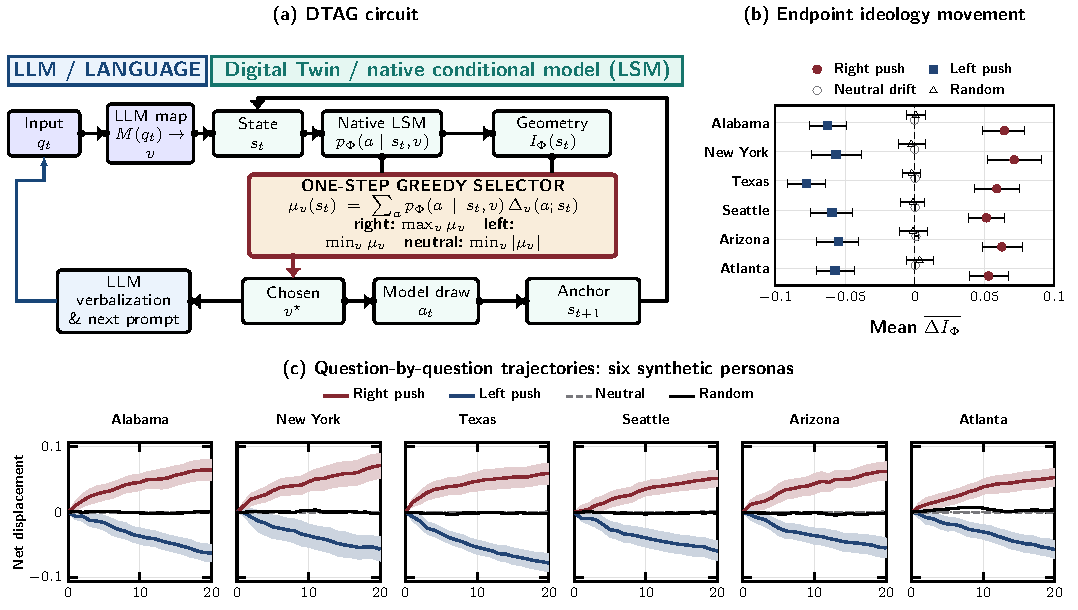
\includegraphics[width=\textwidth]{Figures/External/dtag-fig1}

\vspace{-10pt}

\caption{\textbf{DTAG architecture and native adaptive results.}
(a) LSM-anchored responses and directional question selection; language mapping is a separate interface.
(b) Mean endpoint displacement across six personas with 95\% bootstrap intervals.
(c) Mean \DTAGSteps{}-question trajectories over \DTAGReps{} repetitions per persona and policy, with pointwise 95\% intervals (right: red; left: blue; neutral: dashed gray; random: black).}
\label{fig:arch_adaptive}
\label{fig:arch}
\label{fig:persona-endpoints}
\label{fig:native-trajectories}
\end{figure*}

\section{Adaptive Question Selection}
A semantic interface can map a natural-language question $q$ to a survey item $v\in M(q)$ and verbalize its answer. The native experiments use item identifiers directly without the LLM layer. For a selected question, DTAG samples a response and updates the predictive phenotype:
\begin{align}
A_t&\sim p_\Ph(\cdot\mid s_t,v_t),\label{eq:draw}\\
s_{t+1}&=s_t\cup\{v_t=A_t\},\label{eq:update}\\
\calB_{t+1}&=\calB_\Ph(s_{t+1}).\label{eq:posterior}
\end{align}
The initial persona anchors remain fixed. The optimizer chooses the question, not its answer (Fig.~\ref{fig:arch_adaptive}).

For candidate item $v$ and answer $a$, define
\begin{align}
\Delta_v(a;s)&=I_\Ph(s\cup\{v=a\})-I_\Ph(s),\label{eq:delta}\\
\mu_v(s)&=\sum_{a\in\mathcal A_v}p_\Ph(a\mid s,v)\Delta_v(a;s),\label{eq:mu}\\
\sigma_v^2(s)&=\sum_a p_\Ph(a\mid s,v)(\Delta_v(a;s)-\mu_v(s))^2.
\label{eq:var}
\end{align}
Right- and left-seeking policies maximize and minimize $\mu_v(s)$; neutral minimizes $|\mu_v(s)|$, and random samples an eligible item. By construction,
\begin{equation*}
\EE[I_\Ph(s_{t+1})-I_\Ph(s_t)\mid s_t,v_t]=\mu_{v_t}(s_t).
\end{equation*}
The accumulated displacement depends on successive selected items and sampled answers.

The effect on an unasked item $j$ after observing $(v,a)$ is
\begin{equation}
R_j(s;v,a)=\JS\!\bigl(p_\Ph(\cdot\mid s,j),
p_\Ph(\cdot\mid s\cup\{v=a\},j)\bigr).
\label{eq:ripple}
\end{equation}
A weighted sum $\mathcal P_\Ph(s;v,a)=\sum_{j\notin S\cup\{v\}}w_jR_j(s;v,a)$ measures redistribution across the remaining items. Unlike text retrieval \cite{lewis2020}, DTAG maintains an explicit conditional response state. The public implementation includes a web application (\url{https://github.com/zeroknowledgediscovery/DTAG/tree/main/webapp}).

\section{Refinement and Possible Response Effects}
Under \emph{phenotypic refinement}, successive answers restrict predictions for unasked items. For held-out responses $Y$, the expected information from asking $v$ is
\begin{equation}
\mathcal G(v\mid s)=
H(Y\mid s)-\EE_{A_v\mid s}[H(Y\mid s,v=A_v)].
\label{eq:ig}
\end{equation}
Under a coherent joint model this is conditional mutual information, distinct from directional displacement $\mu_v(s)$. Held-out response prediction evaluates refinement directly.

\begin{table*}[!t]
\centering
\caption{Pinned GSS 2024 synthetic personas and baseline pole-relative index.}
\label{tab:personas}
\begingroup
\small
\footnotesize
\renewcommand{\arraystretch}{1.06}
\begin{tabularx}{\textwidth}{@{}p{.75in}X>{\raggedleft\arraybackslash}p{.90in}@{}}
\toprule
\textbf{Persona} & \textbf{Pinned description} & \textbf{Initial $I_\Phi(s_0)$} \\
\midrule
Alabama & 45-year-old rural Alabama white man; married, two children; full-time farmer and veteran; high school; conservative, strong Republican; Protestant, weekly attendance; daily newspaper. & $0.075706$ \\
\addlinespace[2pt]
New York & 22-year-old New York City white woman; unmarried, no children; full-time retail worker, nonveteran; bachelor's degree; extremely liberal, strong Democrat; nonreligious; daily newspaper. & $-0.163807$ \\
\addlinespace[2pt]
Texas & 61-year-old small-town Texas white woman; married, three children; homemaker, high school; extremely conservative, strong Republican; Protestant, attends services several times weekly; daily newspaper. & $0.045379$ \\
\addlinespace[2pt]
Seattle & 34-year-old Seattle white man; unmarried, no children; employed full time, graduate degree; liberal, weak Democrat; nonreligious; newspaper several times weekly. & $-0.119639$ \\
\addlinespace[2pt]
Arizona & 39-year-old Mexican American man in an Arizona city; married, three children; employed full time, high school; conservative, weak Republican; Catholic, nearly weekly attendance. & $-0.020437$ \\
\addlinespace[2pt]
Atlanta & 47-year-old Atlanta Black woman; divorced, two children; employed full time, bachelor's degree; liberal, strong Democrat; Protestant, weekly attendance; daily newspaper. & $-0.030807$ \\
\bottomrule
\end{tabularx}
\endgroup
\vspace{2pt}

{\footnotesize\raggedright Positive values lie nearer the right reference pole; negative values nearer the left.\par}
\end{table*}

\begin{figure*}[!ht]
\centering
\tikzsetnextfilename{dtag-fig2}
\tikzexternalenable
%\noindent\makebox[\textwidth]{%
  \makebox[.38\textwidth]{\small\bfseries (a) Question identities}%
  \hfill
  \makebox[.59\textwidth]{\small\bfseries (b) Fixed-order displacement}%
}\par\vspace{1mm}
% Two independent TikZ pictures, side by side. No nested wrappers.
%\resizebox{\textwidth}{!}{%
\begin{tikzpicture}[font=\bf\sffamily\fontsize{9}{9}\selectfont]
\node[] (A) at (0,0) {
\begin{tikzpicture}[anchor=center]
\tikzpicturedependsonfile{\DTAGMetadataCSV}
\tikzpicturedependsonfile{\DTAGCSVFigureTwoAF}
\tikzpicturedependsonfile{\DTAGCSVFigureTwoAD}
\tikzpicturedependsonfile{\DTAGCSVFigureTwoAE}
\tikzpicturedependsonfile{\DTAGCSVFigureTwoAR}
\tikzpicturedependsonfile{\DTAGCSVFigureTwoAP}
\tikzpicturedependsonfile{\DTAGCSVFigureTwoAQ}
\tikzpicturedependsonfile{\DTAGCSVFigureTwoAL}
\tikzpicturedependsonfile{\DTAGCSVFigureTwoAJ}
\tikzpicturedependsonfile{\DTAGCSVFigureTwoAK}
\tikzpicturedependsonfile{\DTAGCSVFigureTwoAO}
\tikzpicturedependsonfile{\DTAGCSVFigureTwoAM}
\tikzpicturedependsonfile{\DTAGCSVFigureTwoAN}
\tikzpicturedependsonfile{\DTAGCSVFigureTwoAI}
\tikzpicturedependsonfile{\DTAGCSVFigureTwoAG}
\tikzpicturedependsonfile{\DTAGCSVFigureTwoAH}
\tikzpicturedependsonfile{\DTAGCSVFigureTwoAC}
\tikzpicturedependsonfile{\DTAGCSVFigureTwoAA}
\tikzpicturedependsonfile{\DTAGCSVFigureTwoAB}
\begin{groupplot}[
 group style={group size=3 by 6,horizontal sep=.3cm,vertical sep=.3cm},
 scale only axis,publication axis,
 width=.9in,height=.9in,xmin=.5,xmax=\DTAGXMax,ymin=.5,ymax=\DTAGYMax,
 y dir=reverse,axis on top,xtick={1,\DTAGHalfSteps,\DTAGSteps},ytick={1,\DTAGHalfReps,\DTAGReps},
 xticklabel style={font=\bf\sffamily\fontsize{9}{9}\selectfont},yticklabel style={font=\bf\sffamily\fontsize{9}{9}\selectfont},
 colormap={questionmap}{
   rgb255=(178,24,43)
   rgb255=(239,138,98);
   rgb255=(253,219,199);
   rgb255=(247,247,247);
   rgb255=(209,229,240);
   rgb255=(103,169,207);
   rgb255=(33,102,172);
},
 point meta min=1,point meta max=\DTAGIdMax
]
\nextgroupplot[title={Right push},ylabel={Alabama},xticklabels={}]
\addplot[matrix plot*,mesh/cols=\DTAGSteps,point meta=explicit,mark=none,draw=none] table[x=x,y=y,meta=value,col sep=comma]{\DTAGCSVFigureTwoAF};
\nextgroupplot[title={Left push},yticklabels={},xticklabels={}]
\addplot[matrix plot*,mesh/cols=\DTAGSteps,point meta=explicit,mark=none,draw=none] table[x=x,y=y,meta=value,col sep=comma]{\DTAGCSVFigureTwoAD};
\nextgroupplot[title={Neutral},yticklabels={},xticklabels={}]
\addplot[matrix plot*,mesh/cols=\DTAGSteps,point meta=explicit,mark=none,draw=none] table[x=x,y=y,meta=value,col sep=comma]{\DTAGCSVFigureTwoAE};
\nextgroupplot[ylabel={New York},xticklabels={}]
\addplot[matrix plot*,mesh/cols=\DTAGSteps,point meta=explicit,mark=none,draw=none] table[x=x,y=y,meta=value,col sep=comma]{\DTAGCSVFigureTwoAR};
\nextgroupplot[yticklabels={},xticklabels={}]
\addplot[matrix plot*,mesh/cols=\DTAGSteps,point meta=explicit,mark=none,draw=none] table[x=x,y=y,meta=value,col sep=comma]{\DTAGCSVFigureTwoAP};
\nextgroupplot[yticklabels={},xticklabels={}]
\addplot[matrix plot*,mesh/cols=\DTAGSteps,point meta=explicit,mark=none,draw=none] table[x=x,y=y,meta=value,col sep=comma]{\DTAGCSVFigureTwoAQ};
\nextgroupplot[ylabel={Texas},xticklabels={}]
\addplot[matrix plot*,mesh/cols=\DTAGSteps,point meta=explicit,mark=none,draw=none] table[x=x,y=y,meta=value,col sep=comma]{\DTAGCSVFigureTwoAL};
\nextgroupplot[yticklabels={},xticklabels={}]
\addplot[matrix plot*,mesh/cols=\DTAGSteps,point meta=explicit,mark=none,draw=none] table[x=x,y=y,meta=value,col sep=comma]{\DTAGCSVFigureTwoAJ};
\nextgroupplot[yticklabels={},xticklabels={},
colorbar,
colorbar style={
 at={(1.18,0.5)},anchor=west,height=4in,width=.24cm,
 title={Question ID},
 title style={font=\scriptsize\bfseries,text=black,rotate=90, anchor=west},
 ytick={1,80,\DTAGIdMax},
 yticklabel style={font=\scriptsize\bfseries,text=black},
 tick style={draw=black,line width=.8pt},
 axis line style={draw=black,line width=.9pt},
 scaled y ticks=false
}]
\addplot[matrix plot*,mesh/cols=\DTAGSteps,point meta=explicit,mark=none,draw=none] table[x=x,y=y,meta=value,col sep=comma]{\DTAGCSVFigureTwoAK};
\nextgroupplot[ylabel={Seattle},xticklabels={}]
\addplot[matrix plot*,mesh/cols=\DTAGSteps,point meta=explicit,mark=none,draw=none] table[x=x,y=y,meta=value,col sep=comma]{\DTAGCSVFigureTwoAO};
\nextgroupplot[yticklabels={},xticklabels={}]
\addplot[matrix plot*,mesh/cols=\DTAGSteps,point meta=explicit,mark=none,draw=none] table[x=x,y=y,meta=value,col sep=comma]{\DTAGCSVFigureTwoAM};
\nextgroupplot[yticklabels={},xticklabels={}]
\addplot[matrix plot*,mesh/cols=\DTAGSteps,point meta=explicit,mark=none,draw=none] table[x=x,y=y,meta=value,col sep=comma]{\DTAGCSVFigureTwoAN};
\nextgroupplot[ylabel={Arizona},xticklabels={}]
\addplot[matrix plot*,mesh/cols=\DTAGSteps,point meta=explicit,mark=none,draw=none] table[x=x,y=y,meta=value,col sep=comma]{\DTAGCSVFigureTwoAI};
\nextgroupplot[yticklabels={},xticklabels={}]
\addplot[matrix plot*,mesh/cols=\DTAGSteps,point meta=explicit,mark=none,draw=none] table[x=x,y=y,meta=value,col sep=comma]{\DTAGCSVFigureTwoAG};
\nextgroupplot[yticklabels={},xticklabels={}]
\addplot[matrix plot*,mesh/cols=\DTAGSteps,point meta=explicit,mark=none,draw=none] table[x=x,y=y,meta=value,col sep=comma]{\DTAGCSVFigureTwoAH};
\nextgroupplot[ylabel={Atlanta}%% ,xlabel={Position}
]
\addplot[matrix plot*,mesh/cols=\DTAGSteps,point meta=explicit,mark=none,draw=none] table[x=x,y=y,meta=value,col sep=comma]{\DTAGCSVFigureTwoAC};
\nextgroupplot[yticklabels={},xlabel={Question number}]
\addplot[matrix plot*,mesh/cols=\DTAGSteps,point meta=explicit,mark=none,draw=none] table[x=x,y=y,meta=value,col sep=comma]{\DTAGCSVFigureTwoAA};
\nextgroupplot[yticklabels={}%% ,xlabel={Position}
]
\addplot[matrix plot*,mesh/cols=\DTAGSteps,point meta=explicit,mark=none,draw=none] table[x=x,y=y,meta=value,col sep=comma]{\DTAGCSVFigureTwoAB};
\end{groupplot}
\end{tikzpicture}};%
\node[anchor=north west] at (A.north east) {
\begin{tikzpicture}[anchor=center]
\tikzpicturedependsonfile{\DTAGMetadataCSV}
\tikzpicturedependsonfile{\DTAGCSVFigureTwoAX}
\tikzpicturedependsonfile{\DTAGCSVFigureTwoAV}
\tikzpicturedependsonfile{\DTAGCSVFigureTwoAW}
\tikzpicturedependsonfile{\DTAGCSVFigureTwoBJ}
\tikzpicturedependsonfile{\DTAGCSVFigureTwoBH}
\tikzpicturedependsonfile{\DTAGCSVFigureTwoBI}
\tikzpicturedependsonfile{\DTAGCSVFigureTwoBD}
\tikzpicturedependsonfile{\DTAGCSVFigureTwoBB}
\tikzpicturedependsonfile{\DTAGCSVFigureTwoBC}
\tikzpicturedependsonfile{\DTAGCSVFigureTwoBG}
\tikzpicturedependsonfile{\DTAGCSVFigureTwoBE}
\tikzpicturedependsonfile{\DTAGCSVFigureTwoBF}
\tikzpicturedependsonfile{\DTAGCSVFigureTwoBA}
\tikzpicturedependsonfile{\DTAGCSVFigureTwoAY}
\tikzpicturedependsonfile{\DTAGCSVFigureTwoAZ}
\tikzpicturedependsonfile{\DTAGCSVFigureTwoAU}
\tikzpicturedependsonfile{\DTAGCSVFigureTwoAS}
\tikzpicturedependsonfile{\DTAGCSVFigureTwoAT}
\begin{groupplot}[
 group style={group size=3 by 6,horizontal sep=.2in,vertical sep=.72cm},
 publication axis,scale only axis,width=1in,height=.78in,
 xmin=-\DTAGOrderBound,xmax=\DTAGOrderBound,ymin=.5,ymax=3.5,
 ytick={1,2,3},yticklabels={Shuffle 2,Shuffle 1,Reverse},
 xtick={-.04,-.02,0,.02,.04},
 xticklabel={\pgfmathprintnumber[fixed,precision=2]{\tick}},
]
\nextgroupplot[title={Right-derived},ylabel={Alabama},xticklabels={}]
\addplot[black!65,line width=.75pt,forget plot] coordinates{(0,.5)(0,3.5)};
\addplot[black,only marks,mark=*,mark size=2pt,
 error bars/.cd,x dir=both,x explicit,error bar style={black,line width=.95pt},
 error mark options={rotate=90,mark size=1.65pt}]
 table[x=mean,y=y,x error minus=minus,x error plus=plus,col sep=comma]{\DTAGCSVFigureTwoAX};
\nextgroupplot[title={Left-derived},yticklabels={},xticklabels={}]
\addplot[black!65,line width=.75pt,forget plot] coordinates{(0,.5)(0,3.5)};
\addplot[black,only marks,mark=*,mark size=2pt,
 error bars/.cd,x dir=both,x explicit,error bar style={black,line width=.95pt},
 error mark options={rotate=90,mark size=1.65pt}]
 table[x=mean,y=y,x error minus=minus,x error plus=plus,col sep=comma]{\DTAGCSVFigureTwoAV};
\nextgroupplot[title={Neutral-derived},yticklabels={},xticklabels={}]
\addplot[black!65,line width=.75pt,forget plot] coordinates{(0,.5)(0,3.5)};
\addplot[black,only marks,mark=*,mark size=2pt,
 error bars/.cd,x dir=both,x explicit,error bar style={black,line width=.95pt},
 error mark options={rotate=90,mark size=1.65pt}]
 table[x=mean,y=y,x error minus=minus,x error plus=plus,col sep=comma]{\DTAGCSVFigureTwoAW};
\nextgroupplot[ylabel={New York},xticklabels={}]
\addplot[black!65,line width=.75pt,forget plot] coordinates{(0,.5)(0,3.5)};
\addplot[black,only marks,mark=*,mark size=2pt,
 error bars/.cd,x dir=both,x explicit,error bar style={black,line width=.95pt},
 error mark options={rotate=90,mark size=1.65pt}]
 table[x=mean,y=y,x error minus=minus,x error plus=plus,col sep=comma]{\DTAGCSVFigureTwoBJ};
\nextgroupplot[yticklabels={},xticklabels={}]
\addplot[black!65,line width=.75pt,forget plot] coordinates{(0,.5)(0,3.5)};
\addplot[black,only marks,mark=*,mark size=2pt,
 error bars/.cd,x dir=both,x explicit,error bar style={black,line width=.95pt},
 error mark options={rotate=90,mark size=1.65pt}]
 table[x=mean,y=y,x error minus=minus,x error plus=plus,col sep=comma]{\DTAGCSVFigureTwoBH};
\nextgroupplot[yticklabels={},xticklabels={}]
\addplot[black!65,line width=.75pt,forget plot] coordinates{(0,.5)(0,3.5)};
\addplot[black,only marks,mark=*,mark size=2pt,
 error bars/.cd,x dir=both,x explicit,error bar style={black,line width=.95pt},
 error mark options={rotate=90,mark size=1.65pt}]
 table[x=mean,y=y,x error minus=minus,x error plus=plus,col sep=comma]{\DTAGCSVFigureTwoBI};
\nextgroupplot[ylabel={Texas},xticklabels={}]
\addplot[black!65,line width=.75pt,forget plot] coordinates{(0,.5)(0,3.5)};
\addplot[black,only marks,mark=*,mark size=2pt,
 error bars/.cd,x dir=both,x explicit,error bar style={black,line width=.95pt},
 error mark options={rotate=90,mark size=1.65pt}]
 table[x=mean,y=y,x error minus=minus,x error plus=plus,col sep=comma]{\DTAGCSVFigureTwoBD};
\nextgroupplot[yticklabels={},xticklabels={}]
\addplot[black!65,line width=.75pt,forget plot] coordinates{(0,.5)(0,3.5)};
\addplot[black,only marks,mark=*,mark size=2pt,
 error bars/.cd,x dir=both,x explicit,error bar style={black,line width=.95pt},
 error mark options={rotate=90,mark size=1.65pt}]
 table[x=mean,y=y,x error minus=minus,x error plus=plus,col sep=comma]{\DTAGCSVFigureTwoBB};
\nextgroupplot[yticklabels={},xticklabels={}]
\addplot[black!65,line width=.75pt,forget plot] coordinates{(0,.5)(0,3.5)};
\addplot[black,only marks,mark=*,mark size=2pt,
 error bars/.cd,x dir=both,x explicit,error bar style={black,line width=.95pt},
 error mark options={rotate=90,mark size=1.65pt}]
 table[x=mean,y=y,x error minus=minus,x error plus=plus,col sep=comma]{\DTAGCSVFigureTwoBC};
\nextgroupplot[ylabel={Seattle},xticklabels={}]
\addplot[black!65,line width=.75pt,forget plot] coordinates{(0,.5)(0,3.5)};
\addplot[black,only marks,mark=*,mark size=2pt,
 error bars/.cd,x dir=both,x explicit,error bar style={black,line width=.95pt},
 error mark options={rotate=90,mark size=1.65pt}]
 table[x=mean,y=y,x error minus=minus,x error plus=plus,col sep=comma]{\DTAGCSVFigureTwoBG};
\nextgroupplot[yticklabels={},xticklabels={}]
\addplot[black!65,line width=.75pt,forget plot] coordinates{(0,.5)(0,3.5)};
\addplot[black,only marks,mark=*,mark size=2pt,
 error bars/.cd,x dir=both,x explicit,error bar style={black,line width=.95pt},
 error mark options={rotate=90,mark size=1.65pt}]
 table[x=mean,y=y,x error minus=minus,x error plus=plus,col sep=comma]{\DTAGCSVFigureTwoBE};
\nextgroupplot[yticklabels={},xticklabels={}]
\addplot[black!65,line width=.75pt,forget plot] coordinates{(0,.5)(0,3.5)};
\addplot[black,only marks,mark=*,mark size=2pt,
 error bars/.cd,x dir=both,x explicit,error bar style={black,line width=.95pt},
 error mark options={rotate=90,mark size=1.65pt}]
 table[x=mean,y=y,x error minus=minus,x error plus=plus,col sep=comma]{\DTAGCSVFigureTwoBF};
\nextgroupplot[ylabel={Arizona},xticklabels={}]
\addplot[black!65,line width=.75pt,forget plot] coordinates{(0,.5)(0,3.5)};
\addplot[black,only marks,mark=*,mark size=2pt,
 error bars/.cd,x dir=both,x explicit,error bar style={black,line width=.95pt},
 error mark options={rotate=90,mark size=1.65pt}]
 table[x=mean,y=y,x error minus=minus,x error plus=plus,col sep=comma]{\DTAGCSVFigureTwoBA};
\nextgroupplot[yticklabels={},xticklabels={}]
\addplot[black!65,line width=.75pt,forget plot] coordinates{(0,.5)(0,3.5)};
\addplot[black,only marks,mark=*,mark size=2pt,
 error bars/.cd,x dir=both,x explicit,error bar style={black,line width=.95pt},
 error mark options={rotate=90,mark size=1.65pt}]
 table[x=mean,y=y,x error minus=minus,x error plus=plus,col sep=comma]{\DTAGCSVFigureTwoAY};
\nextgroupplot[yticklabels={},xticklabels={}]
\addplot[black!65,line width=.75pt,forget plot] coordinates{(0,.5)(0,3.5)};
\addplot[black,only marks,mark=*,mark size=2pt,
 error bars/.cd,x dir=both,x explicit,error bar style={black,line width=.95pt},
 error mark options={rotate=90,mark size=1.65pt}]
 table[x=mean,y=y,x error minus=minus,x error plus=plus,col sep=comma]{\DTAGCSVFigureTwoAZ};
\nextgroupplot[ylabel={Atlanta},%% xlabel={$I_{20}-I_0$}
]
\addplot[black!65,line width=.75pt,forget plot] coordinates{(0,.5)(0,3.5)};
\addplot[black,only marks,mark=*,mark size=2pt,
 error bars/.cd,x dir=both,x explicit,error bar style={black,line width=.95pt},
 error mark options={rotate=90,mark size=1.65pt}]
 table[x=mean,y=y,x error minus=minus,x error plus=plus,col sep=comma]{\DTAGCSVFigureTwoAU};
\nextgroupplot[yticklabels={},xlabel={$I_{20}-I_0$}]
\addplot[black!65,line width=.75pt,forget plot] coordinates{(0,.5)(0,3.5)};
\addplot[black,only marks,mark=*,mark size=2pt,
 error bars/.cd,x dir=both,x explicit,error bar style={black,line width=.95pt},
 error mark options={rotate=90,mark size=1.65pt}]
 table[x=mean,y=y,x error minus=minus,x error plus=plus,col sep=comma]{\DTAGCSVFigureTwoAS};
\nextgroupplot[yticklabels={}%% ,xlabel={$I_{20}-I_0$}
]
\addplot[black!65,line width=.75pt,forget plot] coordinates{(0,.5)(0,3.5)};
\addplot[black,only marks,mark=*,mark size=2pt,
 error bars/.cd,x dir=both,x explicit,error bar style={black,line width=.95pt},
 error mark options={rotate=90,mark size=1.65pt}]
 table[x=mean,y=y,x error minus=minus,x error plus=plus,col sep=comma]{\DTAGCSVFigureTwoAT};
\end{groupplot}
\end{tikzpicture}};%
\end{tikzpicture}


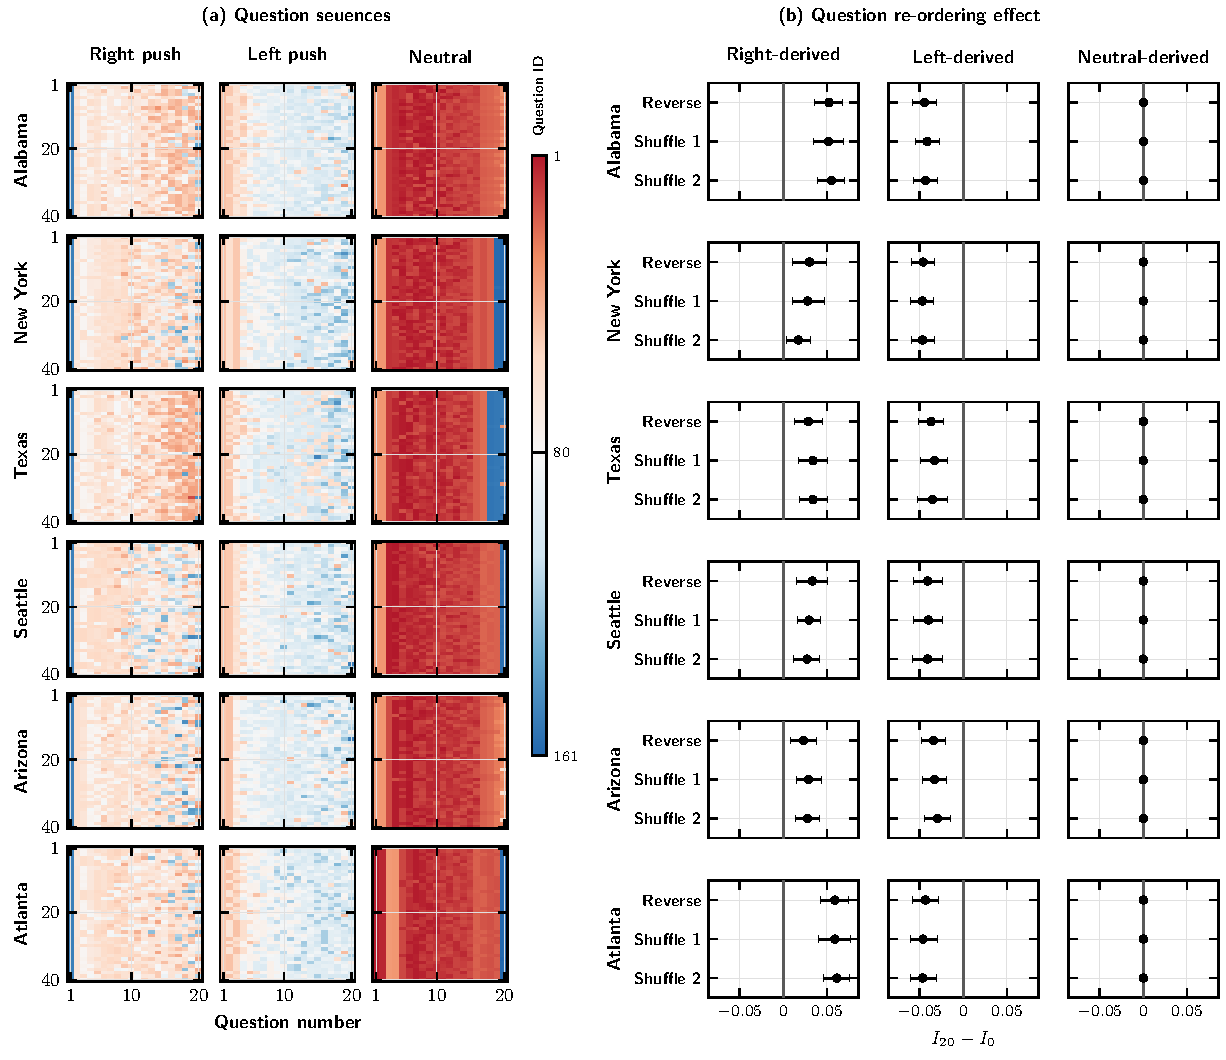
\includegraphics[width=\textwidth]{Figures/External/dtag-fig2}

\vspace{-10pt}

\caption{\textbf{Selected questions and fixed-set replays.}
Left: question-ID heatmaps for six personas and three selection policies (\DTAGReps{} runs each); color denotes item identity.
Right: mean index displacement and 95\% bootstrap intervals for 20-item sets replayed in original, reversed, and two shuffled orders. Right- and left-derived sets retain their direction; neutral sets remain near zero.}
\label{fig:question-map}
\label{fig:order-effects}
\end{figure*}
\subsection{Possible response effects.}
Questioning a person may change later reports. A response--transition kernel separates an observed answer from a possible latent-state update:
\begin{equation}
K_q(a,z'\mid z)=O_q(a\mid z)\,T_q(z'\mid z,a).
\label{eq:kernel}
\end{equation}
Passive observation has $T_q(z'\mid z,a)=\delta_z(z')$; shifts in salience or belief can induce nontrivial transitions. A common held-out battery and delayed measurement can investigate these effects.

\subsection{Order dependence.}
For fixed realized answers, the terminal index is order-independent; sequentially generated answers need not be. A coherent joint distribution satisfies
\begin{equation}
P(a\mid s,v)P(b\mid s,v=a,w)
=P(b\mid s,w)P(a\mid s,w=b,v).
\label{eq:compat}
\end{equation}
Separately fitted LSM conditionals may violate this identity \cite{heckerman2000}. Fixed-set replays evaluate its consequences for native response sequences.

\section{Native GSS 2024 Computational Experiments}
\label{sec:native}

\subsection{Adaptive questioning from pinned persona states}
We fixed six initial GSS 2024 persona states (Table~\ref{tab:personas}) and generated 40 independent response sequences per persona and policy (right, left, neutral, random). Each sequence comprised 20 questions with responses sampled from the native LSM; no LLM mapping or verbalization was used. \emph{All 27 pole-defining items were excluded from selection in every policy} (Table~\ref{tab:poles}). Thus 960 adaptive trajectories contain 19,200 non-pole responses; repetitions share initial anchors but have independent sampled answers.




Across all six personas, right- and left-seeking policies moved the index in their intended directions (Fig.~\ref{fig:arch_adaptive}). As pole-defining questions were excluded, the movement results from conditioning on other survey items, not directly asking those used to define the reference index. Neutral and random policies provide comparisons.

\begin{table}[!t]
\centering
\caption{Question selection in the native GSS 2024 experiment.}
\label{tab:question-coverage}
\begingroup
\footnotesize
\setlength{\tabcolsep}{4pt}
\renewcommand{\arraystretch}{1.08}
\begin{tabular}{@{}lrrr@{}}
\toprule
\textbf{Selection policy} & \textbf{Distinct} & \textbf{Selections} & \textbf{Pole overlap}\\
\midrule
Right-seeking & 100 & 4,800 & 0\\
Left-seeking & 75 & 4,800 & 0\\
Neutral & 43 & 4,800 & 0\\
\midrule
Three-policy union & 161 & 14,400 & 0\\
All four policies & 228 & 19,200 & 0\\
\bottomrule
\end{tabular}
\endgroup
\par\smallskip
{\footnotesize\raggedright The random policy contributed 4,800 selections; 67 of the 228 distinct items occurred only under random selection.\par}
\end{table}

\subsection{Question selection as observed paths}
Question identities are summarized in Table~\ref{tab:question-coverage}. The 18 displayed heatmaps contain 161 distinct items across right, left, and neutral selection (Fig.~\ref{fig:question-map}). A shared categorical ordering approximately minimizes
\begin{equation}
\mathcal C(\pi)=\sum_{p,u,t}\sum_{r<r'}
\big|\pi(v_{purt})-\pi(v_{pur't})\big|,
\label{eq:question-seriation}
\end{equation}
Here $u$ indexes policies. Heatmap colors identify items, not ideological position; 67 further items occurred only in random selection.



\subsection{Fixed-set replay: robustness to question ordering}
For each persona and right/left/neutral policy, we froze the 20-item sequence from adaptive replicate zero, giving 18 fixed sets. Each set was replayed in original, reversed, and two shuffled orders with 40 fresh sampled responses per order (2,880 runs). Matched question-specific random variates reduced contrast variance.

The direction persisted across replays (Fig.~\ref{fig:order-effects}): right-derived sets yielded mean displacement $+0.0381$ (original) and $+0.0377$ (reversed); left-derived sets yielded $-0.0399$ and $-0.0410$. In both orders, all six persona-specific 95\% bootstrap intervals excluded zero in the prescribed direction. Shuffles followed the same pattern; neutral sets remained near zero.

All 54 pointwise bootstrap intervals for paired mean between-order contrasts included zero; no systematic mean order effect was detected. Selected question sets therefore retained directional displacement without continuous reoptimization.

In historical ten-question runs, baseline indices differed across environments despite matched persona, map, and pole hashes; native binaries were not compared. Their absolute indices are not combined with the present experiment.


\section{Human Study: Hypothesis and Validation}
Our hypothesis is that adaptive questioning can \emph{steer the inferred ideology index toward a specified pole}, with directional movement relative to the respondent's own baseline rather than requiring a particular starting ideology. Thus left-seeking questioning should give $\Delta I_\Ph=I_\Ph(s_{20})-I_\Ph(s_0)<0$, and right-seeking questioning should give $\Delta I_\Ph>0$, across heterogeneous initial index values. Neutral and random policies provide non-directional comparisons.

We tested this in 34 completed human sessions with six common baseline questions and twenty adaptive questions (plus five attention checks): Left ($n=5$), Right ($n=17$), Neutral ($n=7$), and Random ($n=5$). Mean endpoint movements were $-0.0783$ for Left and $+0.0382$ for Right, with both 95\% participant-bootstrap intervals excluding zero; Neutral ($-0.0054$) and Random ($-0.0045$) remained near zero. Right-policy respondents spanned both sides of the baseline ideology coordinate (11 negative, 6 positive), directly testing directional movement in a mixed-baseline cohort.


% Human DTAG experiment. Four policy groups only: Left, Right, Neutral, Random.
% Figures/table: python3 human_study/scripts/render_humanstudy_pgfplots.py
% Include from DTAG_main.tex (which already uses % Human DTAG experiment. Four policy groups only: Left, Right, Neutral, Random.
% Figures/table: python3 human_study/scripts/render_humanstudy_pgfplots.py
% Include from DTAG_main.tex (which already uses % Human DTAG experiment. Four policy groups only: Left, Right, Neutral, Random.
% Figures/table: python3 human_study/scripts/render_humanstudy_pgfplots.py
% Include from DTAG_main.tex (which already uses \input{humanstudy}).
% All numbers and confidence intervals in the figures/table are curated
% from immutable GCS records, not illustrative or generated synthetically.

\section{Human Response Study}\label{sec:humanstudy}

\subsection{Protocol and outcome}
We conducted a prospective human-response study, recruiting participants
through Prolific, an established online research-participation platform
\cite{prolificEthics2026}, to evaluate whether adaptive question-selection
policies produce predictable displacement in the pole-relative LSM index.
Participants provided informed consent before answering questions in the
linked DTAG web application. Each participant completed six common
baseline questions, up to twenty adaptive questions, and five interleaved
attention checks. Participants responded in natural language; accepted
survey-variable interpretations were incorporated into the conditional
LSM state. The policy groups are \emph{Left}, \emph{Right},
\emph{Neutral}, and \emph{Random}. Each session contributes to exactly
one of these four groups.

Let $s_0$ denote the conditional state after the six baseline responses
and $s_t$ the state after $t$ adaptive answers. The outcome at each
step is the change in the fixed pole-relative geometric coordinate,
\begin{equation}
\Delta I_\Phi(t)=I_\Phi(s_t)-I_\Phi(s_0),\qquad t=0,\ldots,20.
\label{eq:humanstudy-delta}
\end{equation}
A positive displacement is rightward in this model-defined coordinate
and a negative displacement is leftward. The index measures the inferred survey-response phenotype and makes
directional movement comparable across different baseline positions.

\subsection{Participant characteristics and completion}
Table~\ref{tab:humanstudy-participants} reports, for each of the four
policies, the number of participants who completed the twenty adaptive
questions, the number whose baseline index is negative or positive,
and the mean completion time. Completion time is elapsed wall-clock
time between the session creation timestamp and archived finalization,
and includes the baseline, adaptive questions, attention checks, and
any waits between responses. All table entries are derived directly
from immutable completed-session records rather than estimated from
the number of questions.

\begin{table*}[!t]
\centering
\caption{Human study summary by adaptive question-selection policy$^\star$.
}
\label{tab:humanstudy-participants}
\small
\setlength{\tabcolsep}{11pt}
\begin{tabular}{lrrrr}
\toprule
Policy & Completed $n$ & Baseline $I_\Phi<0$ & Baseline $I_\Phi>0$ & Mean completion (min) \\
\midrule
Left & 5 & 5 & 0 & 36.7 \\
Right & 17 & 11 & 6 & 34.3 \\
Neutral & 7 & 6 & 1 & 30.8 \\
Random & 5 & 2 & 3 & 35.3 \\
\bottomrule
\end{tabular}
\flushleft $^\star$Completion time is wall-clock time from session creation to finalization,
including baseline questions, adaptive questions, and attention checks.
Baseline signs refer to the LSM-derived ideology coordinate before
adaptive questioning.
\end{table*}

\subsection{Question-by-question trajectories and endpoints}
Figure~\ref{fig:humanstudy-trajectory-endpoints}(a) plots mean
$\Delta I_\Phi(t)$ for all four policies. For a given question number,
the mean includes only participants with an observed answer at that
step. A participant who did not finish contributes only through their
last recorded answer, with no interpolation, imputation, or endpoint
carry-forward. The shaded regions are pointwise 95\% confidence
intervals from participant-level bootstrap resampling (5{,}000
replicates by default). For clarity, \emph{only Left and Right} carry
shaded intervals; Neutral and Random are shown as mean trajectories.

Figure~\ref{fig:humanstudy-trajectory-endpoints}(b) reports the
question-20 endpoint for \emph{all four} policies, each as a mean
and a 95\% participant-bootstrap confidence interval. Unlike the
stepwise trajectories, endpoint estimates use only participants with
all twenty adaptive questions recorded. The zero reference is no
change relative to baseline. The legend lists only the four policy
names, and participant counts appear separately in
Table~\ref{tab:humanstudy-participants}.



\begin{figure*}[!ht]
\centering
\tikzsetnextfilename{humanstudy}
\tikzexternalenable
\input{Figures/humanstudy_figures}

%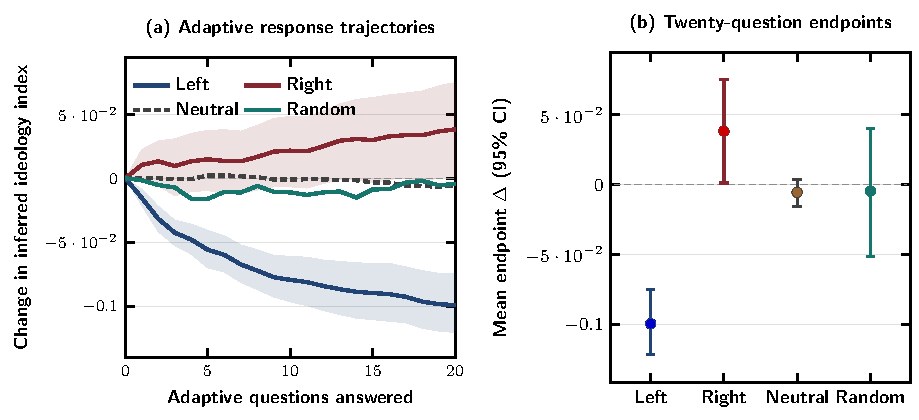
\includegraphics[width=\textwidth]{Figures/External/humanstudy}

\vspace{-10pt}
\caption{\textbf{Human study response trajectories and endpoints.}
(a) The mean change from baseline in the LSM-derived ideology coordinate as
adaptive questions are answered, with pointwise 95\% participant-bootstrap
confidence intervals shaded only for Left and Right. Partial sessions contribute
only through their last observed step. (b) Endpoint means and 95\% bootstrap
confidence intervals for all four policies, calculated from participants with
all 20 adaptive answers. Arm sample sizes are reported in
Table~\ref{tab:humanstudy-participants}.}
\label{fig:humanstudy-trajectory-endpoints}


\end{figure*}



\subsection{Interpretation}
The human results support the directional-steering hypothesis. At
question 20, Left moved the inferred ideology index by $-0.0783$
(95\% bootstrap CI $[-0.1130,-0.0195]$), and Right moved it by
$+0.0382$ (CI $[+0.0012,+0.0748]$). Neutral ($-0.0054$) and
Random ($-0.0045$) showed substantially smaller mean changes.
The Right arm included 11 participants with negative and six with
positive baseline indices; rightward mean movement therefore occurred
in a cohort spanning both sides of the initial ideology coordinate.

Together with the native simulations, these human-response results
demonstrate directional control over the \emph{inferred ideology
index} through adaptive question selection. Defining displacement
relative to each participant's own baseline allows this effect to
be evaluated across heterogeneous starting states.
).
% All numbers and confidence intervals in the figures/table are curated
% from immutable GCS records, not illustrative or generated synthetically.

\section{Human Response Study}\label{sec:humanstudy}

\subsection{Protocol and outcome}
We conducted a prospective human-response study, recruiting participants
through Prolific, an established online research-participation platform
\cite{prolificEthics2026}, to evaluate whether adaptive question-selection
policies produce predictable displacement in the pole-relative LSM index.
Participants provided informed consent before answering questions in the
linked DTAG web application. Each participant completed six common
baseline questions, up to twenty adaptive questions, and five interleaved
attention checks. Participants responded in natural language; accepted
survey-variable interpretations were incorporated into the conditional
LSM state. The policy groups are \emph{Left}, \emph{Right},
\emph{Neutral}, and \emph{Random}. Each session contributes to exactly
one of these four groups.

Let $s_0$ denote the conditional state after the six baseline responses
and $s_t$ the state after $t$ adaptive answers. The outcome at each
step is the change in the fixed pole-relative geometric coordinate,
\begin{equation}
\Delta I_\Phi(t)=I_\Phi(s_t)-I_\Phi(s_0),\qquad t=0,\ldots,20.
\label{eq:humanstudy-delta}
\end{equation}
A positive displacement is rightward in this model-defined coordinate
and a negative displacement is leftward. The index measures the inferred survey-response phenotype and makes
directional movement comparable across different baseline positions.

\subsection{Participant characteristics and completion}
Table~\ref{tab:humanstudy-participants} reports, for each of the four
policies, the number of participants who completed the twenty adaptive
questions, the number whose baseline index is negative or positive,
and the mean completion time. Completion time is elapsed wall-clock
time between the session creation timestamp and archived finalization,
and includes the baseline, adaptive questions, attention checks, and
any waits between responses. All table entries are derived directly
from immutable completed-session records rather than estimated from
the number of questions.

\begin{table*}[!t]
\centering
\caption{Human study summary by adaptive question-selection policy$^\star$.
}
\label{tab:humanstudy-participants}
\small
\setlength{\tabcolsep}{11pt}
\begin{tabular}{lrrrr}
\toprule
Policy & Completed $n$ & Baseline $I_\Phi<0$ & Baseline $I_\Phi>0$ & Mean completion (min) \\
\midrule
Left & 5 & 5 & 0 & 36.7 \\
Right & 17 & 11 & 6 & 34.3 \\
Neutral & 7 & 6 & 1 & 30.8 \\
Random & 5 & 2 & 3 & 35.3 \\
\bottomrule
\end{tabular}
\flushleft $^\star$Completion time is wall-clock time from session creation to finalization,
including baseline questions, adaptive questions, and attention checks.
Baseline signs refer to the LSM-derived ideology coordinate before
adaptive questioning.
\end{table*}

\subsection{Question-by-question trajectories and endpoints}
Figure~\ref{fig:humanstudy-trajectory-endpoints}(a) plots mean
$\Delta I_\Phi(t)$ for all four policies. For a given question number,
the mean includes only participants with an observed answer at that
step. A participant who did not finish contributes only through their
last recorded answer, with no interpolation, imputation, or endpoint
carry-forward. The shaded regions are pointwise 95\% confidence
intervals from participant-level bootstrap resampling (5{,}000
replicates by default). For clarity, \emph{only Left and Right} carry
shaded intervals; Neutral and Random are shown as mean trajectories.

Figure~\ref{fig:humanstudy-trajectory-endpoints}(b) reports the
question-20 endpoint for \emph{all four} policies, each as a mean
and a 95\% participant-bootstrap confidence interval. Unlike the
stepwise trajectories, endpoint estimates use only participants with
all twenty adaptive questions recorded. The zero reference is no
change relative to baseline. The legend lists only the four policy
names, and participant counts appear separately in
Table~\ref{tab:humanstudy-participants}.



\begin{figure*}[!ht]
\centering
\tikzsetnextfilename{humanstudy}
\tikzexternalenable
% Human DTAG empirical panels. All coordinates are read from curated CSVs.
% Generated by: python3 human_study/scripts/render_humanstudy_pgfplots.py
% Compile from within tex/ using DTAG_main.tex.
% Styles follow DTAG figures 1--2: publication axis, bold labels and strong ticks.
\begin{figure*}[!t]
\centering
\begin{minipage}[t]{0.605\textwidth}
\centering
{\small\sffamily\bfseries (a) Adaptive response trajectories}\par\vspace{1.0mm}
\begin{tikzpicture}
\begin{axis}[
  publication axis,
  width=\linewidth, height=0.35\textwidth,
  scale only axis=false,
  xmin=0, xmax=20,
  xtick={0,5,10,15,20},
  xlabel={Adaptive questions answered},
  ylabel={Change in inferred ideology index},
  axis line style={black,line width=1pt},
  tick style={black,line width=.95pt},
  tick label style={font=\footnotesize\bfseries},
  label style={font=\small\bfseries},
  legend style={draw=none,fill=none,font=\small\bfseries,at={(0.02,0.98)},anchor=north west},
  legend cell align=left,
  ymajorgrids, grid style={black!12,line width=.3pt}
]
\addplot[black!45,densely dashed,thin,forget plot] coordinates {(0,0) (20,0)};
% Participant-level 95% confidence bands only for Left and Right.
\addplot[name path=hsleftlo,draw=none,forget plot]
  table[x=step,y=ci_low,col sep=comma]{Figures/humanstudy_trajectory_left.csv};
\addplot[name path=hslefthi,draw=none,forget plot]
  table[x=step,y=ci_high,col sep=comma]{Figures/humanstudy_trajectory_left.csv};
\addplot[fill=dtblue,fill opacity=.14,draw=none,forget plot]
  fill between[of=hsleftlo and hslefthi];
\addplot[name path=hsrightlo,draw=none,forget plot]
  table[x=step,y=ci_low,col sep=comma]{Figures/humanstudy_trajectory_right.csv};
\addplot[name path=hsrighthi,draw=none,forget plot]
  table[x=step,y=ci_high,col sep=comma]{Figures/humanstudy_trajectory_right.csv};
\addplot[fill=dtred,fill opacity=.14,draw=none,forget plot]
  fill between[of=hsrightlo and hsrighthi];
\addplot[dtblue,very thick]
  table[x=step,y=mean,col sep=comma]{Figures/humanstudy_trajectory_left.csv};
\addlegendentry{Left}
\addplot[dtred,very thick]
  table[x=step,y=mean,col sep=comma]{Figures/humanstudy_trajectory_right.csv};
\addlegendentry{Right}
\addplot[black!75,very thick]
  table[x=step,y=mean,col sep=comma]{Figures/humanstudy_trajectory_neutral.csv};
\addlegendentry{Neutral}
\addplot[modteal,very thick]
  table[x=step,y=mean,col sep=comma]{Figures/humanstudy_trajectory_random.csv};
\addlegendentry{Random}
\end{axis}
\end{tikzpicture}
\end{minipage}
\hfill
\begin{minipage}[t]{0.365\textwidth}
\centering
{\small\sffamily\bfseries (b) Twenty-question endpoints}\par\vspace{1.0mm}
\begin{tikzpicture}
\begin{axis}[
  publication axis,
  width=\linewidth, height=0.35\textwidth,
  scale only axis=false,
  xmin=.45, xmax=4.55,
  xtick={1,2,3,4},
  xticklabels={Left,Right,Neutral,Random},
  x tick label style={font=\scriptsize\bfseries,rotate=0},
  ylabel={Mean endpoint change (95\% CI)},
  axis line style={black,line width=1pt},
  tick style={black,line width=.95pt},
  tick label style={font=\footnotesize\bfseries},
  label style={font=\small\bfseries},
  ymajorgrids, grid style={black!12,line width=.3pt}
]
\addplot[black!45,densely dashed,thin,forget plot] coordinates {(.5,0) (4.5,0)};
% Mean +/- participant-bootstrap 95% CI for each of all four arms.
\addplot+[only marks,mark=*,mark size=2.5pt,color=dtblue,
  error bars/.cd,y dir=both,y explicit,error bar style={line width=1.05pt},
  error mark options={mark size=2pt,line width=1.05pt}]
  table[x=x,y=mean,y error minus=err_minus,y error plus=err_plus,col sep=comma]
    {Figures/humanstudy_endpoint_left.csv};
\addplot+[only marks,mark=*,mark size=2.5pt,color=dtred,
  error bars/.cd,y dir=both,y explicit,error bar style={line width=1.05pt},
  error mark options={mark size=2pt,line width=1.05pt}]
  table[x=x,y=mean,y error minus=err_minus,y error plus=err_plus,col sep=comma]
    {Figures/humanstudy_endpoint_right.csv};
\addplot+[only marks,mark=*,mark size=2.5pt,color=black!75,
  error bars/.cd,y dir=both,y explicit,error bar style={line width=1.05pt},
  error mark options={mark size=2pt,line width=1.05pt}]
  table[x=x,y=mean,y error minus=err_minus,y error plus=err_plus,col sep=comma]
    {Figures/humanstudy_endpoint_neutral.csv};
\addplot+[only marks,mark=*,mark size=2.5pt,color=modteal,
  error bars/.cd,y dir=both,y explicit,error bar style={line width=1.05pt},
  error mark options={mark size=2pt,line width=1.05pt}]
  table[x=x,y=mean,y error minus=err_minus,y error plus=err_plus,col sep=comma]
    {Figures/humanstudy_endpoint_random.csv};
\end{axis}
\end{tikzpicture}
\end{minipage}
\caption{\textbf{Human DTAG response trajectories and endpoints.}
(a) The mean change from baseline in the LSM-derived ideology coordinate as
adaptive questions are answered, with pointwise 95\% participant-bootstrap
confidence intervals shaded only for Left and Right. Partial sessions contribute
only through their last observed step. (b) Endpoint means and 95\% bootstrap
confidence intervals for all four policies, calculated from participants with
all 20 adaptive answers. The intervals are descriptive, not a measure of
persistent attitude change. Arm sample sizes are reported in
Table~\ref{tab:humanstudy-participants}.}
\label{fig:humanstudy-trajectory-endpoints}
\end{figure*}


%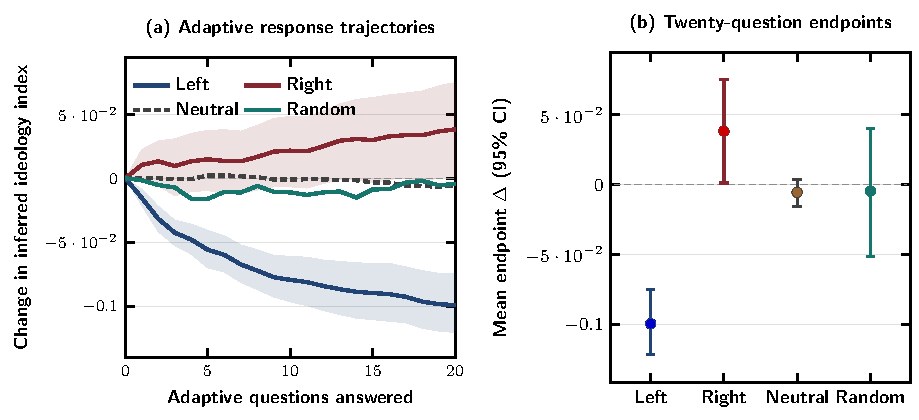
\includegraphics[width=\textwidth]{Figures/External/humanstudy}

\vspace{-10pt}
\caption{\textbf{Human study response trajectories and endpoints.}
(a) The mean change from baseline in the LSM-derived ideology coordinate as
adaptive questions are answered, with pointwise 95\% participant-bootstrap
confidence intervals shaded only for Left and Right. Partial sessions contribute
only through their last observed step. (b) Endpoint means and 95\% bootstrap
confidence intervals for all four policies, calculated from participants with
all 20 adaptive answers. Arm sample sizes are reported in
Table~\ref{tab:humanstudy-participants}.}
\label{fig:humanstudy-trajectory-endpoints}


\end{figure*}



\subsection{Interpretation}
The human results support the directional-steering hypothesis. At
question 20, Left moved the inferred ideology index by $-0.0783$
(95\% bootstrap CI $[-0.1130,-0.0195]$), and Right moved it by
$+0.0382$ (CI $[+0.0012,+0.0748]$). Neutral ($-0.0054$) and
Random ($-0.0045$) showed substantially smaller mean changes.
The Right arm included 11 participants with negative and six with
positive baseline indices; rightward mean movement therefore occurred
in a cohort spanning both sides of the initial ideology coordinate.

Together with the native simulations, these human-response results
demonstrate directional control over the \emph{inferred ideology
index} through adaptive question selection. Defining displacement
relative to each participant's own baseline allows this effect to
be evaluated across heterogeneous starting states.
).
% All numbers and confidence intervals in the figures/table are curated
% from immutable GCS records, not illustrative or generated synthetically.

\section{Human Response Study}\label{sec:humanstudy}

\subsection{Protocol and outcome}
We conducted a prospective human-response study, recruiting participants
through Prolific, an established online research-participation platform
\cite{prolificEthics2026}, to evaluate whether adaptive question-selection
policies produce predictable displacement in the pole-relative LSM index.
Participants provided informed consent before answering questions in the
linked DTAG web application. Each participant completed six common
baseline questions, up to twenty adaptive questions, and five interleaved
attention checks. Participants responded in natural language; accepted
survey-variable interpretations were incorporated into the conditional
LSM state. The policy groups are \emph{Left}, \emph{Right},
\emph{Neutral}, and \emph{Random}. Each session contributes to exactly
one of these four groups.

Let $s_0$ denote the conditional state after the six baseline responses
and $s_t$ the state after $t$ adaptive answers. The outcome at each
step is the change in the fixed pole-relative geometric coordinate,
\begin{equation}
\Delta I_\Phi(t)=I_\Phi(s_t)-I_\Phi(s_0),\qquad t=0,\ldots,20.
\label{eq:humanstudy-delta}
\end{equation}
A positive displacement is rightward in this model-defined coordinate
and a negative displacement is leftward. The index measures the inferred survey-response phenotype and makes
directional movement comparable across different baseline positions.

\subsection{Participant characteristics and completion}
Table~\ref{tab:humanstudy-participants} reports, for each of the four
policies, the number of participants who completed the twenty adaptive
questions, the number whose baseline index is negative or positive,
and the mean completion time. Completion time is elapsed wall-clock
time between the session creation timestamp and archived finalization,
and includes the baseline, adaptive questions, attention checks, and
any waits between responses. All table entries are derived directly
from immutable completed-session records rather than estimated from
the number of questions.

\begin{table*}[!t]
\centering
\caption{Human study summary by adaptive question-selection policy$^\star$.
}
\label{tab:humanstudy-participants}
\small
\setlength{\tabcolsep}{11pt}
\begin{tabular}{lrrrr}
\toprule
Policy & Completed $n$ & Baseline $I_\Phi<0$ & Baseline $I_\Phi>0$ & Mean completion (min) \\
\midrule
Left & 5 & 5 & 0 & 36.7 \\
Right & 17 & 11 & 6 & 34.3 \\
Neutral & 7 & 6 & 1 & 30.8 \\
Random & 5 & 2 & 3 & 35.3 \\
\bottomrule
\end{tabular}
\flushleft $^\star$Completion time is wall-clock time from session creation to finalization,
including baseline questions, adaptive questions, and attention checks.
Baseline signs refer to the LSM-derived ideology coordinate before
adaptive questioning.
\end{table*}

\subsection{Question-by-question trajectories and endpoints}
Figure~\ref{fig:humanstudy-trajectory-endpoints}(a) plots mean
$\Delta I_\Phi(t)$ for all four policies. For a given question number,
the mean includes only participants with an observed answer at that
step. A participant who did not finish contributes only through their
last recorded answer, with no interpolation, imputation, or endpoint
carry-forward. The shaded regions are pointwise 95\% confidence
intervals from participant-level bootstrap resampling (5{,}000
replicates by default). For clarity, \emph{only Left and Right} carry
shaded intervals; Neutral and Random are shown as mean trajectories.

Figure~\ref{fig:humanstudy-trajectory-endpoints}(b) reports the
question-20 endpoint for \emph{all four} policies, each as a mean
and a 95\% participant-bootstrap confidence interval. Unlike the
stepwise trajectories, endpoint estimates use only participants with
all twenty adaptive questions recorded. The zero reference is no
change relative to baseline. The legend lists only the four policy
names, and participant counts appear separately in
Table~\ref{tab:humanstudy-participants}.



\begin{figure*}[!ht]
\centering
\tikzsetnextfilename{humanstudy}
\tikzexternalenable
% Human DTAG empirical panels. All coordinates are read from curated CSVs.
% Generated by: python3 human_study/scripts/render_humanstudy_pgfplots.py
% Compile from within tex/ using DTAG_main.tex.
% Styles follow DTAG figures 1--2: publication axis, bold labels and strong ticks.
\begin{figure*}[!t]
\centering
\begin{minipage}[t]{0.605\textwidth}
\centering
{\small\sffamily\bfseries (a) Adaptive response trajectories}\par\vspace{1.0mm}
\begin{tikzpicture}
\begin{axis}[
  publication axis,
  width=\linewidth, height=0.35\textwidth,
  scale only axis=false,
  xmin=0, xmax=20,
  xtick={0,5,10,15,20},
  xlabel={Adaptive questions answered},
  ylabel={Change in inferred ideology index},
  axis line style={black,line width=1pt},
  tick style={black,line width=.95pt},
  tick label style={font=\footnotesize\bfseries},
  label style={font=\small\bfseries},
  legend style={draw=none,fill=none,font=\small\bfseries,at={(0.02,0.98)},anchor=north west},
  legend cell align=left,
  ymajorgrids, grid style={black!12,line width=.3pt}
]
\addplot[black!45,densely dashed,thin,forget plot] coordinates {(0,0) (20,0)};
% Participant-level 95% confidence bands only for Left and Right.
\addplot[name path=hsleftlo,draw=none,forget plot]
  table[x=step,y=ci_low,col sep=comma]{Figures/humanstudy_trajectory_left.csv};
\addplot[name path=hslefthi,draw=none,forget plot]
  table[x=step,y=ci_high,col sep=comma]{Figures/humanstudy_trajectory_left.csv};
\addplot[fill=dtblue,fill opacity=.14,draw=none,forget plot]
  fill between[of=hsleftlo and hslefthi];
\addplot[name path=hsrightlo,draw=none,forget plot]
  table[x=step,y=ci_low,col sep=comma]{Figures/humanstudy_trajectory_right.csv};
\addplot[name path=hsrighthi,draw=none,forget plot]
  table[x=step,y=ci_high,col sep=comma]{Figures/humanstudy_trajectory_right.csv};
\addplot[fill=dtred,fill opacity=.14,draw=none,forget plot]
  fill between[of=hsrightlo and hsrighthi];
\addplot[dtblue,very thick]
  table[x=step,y=mean,col sep=comma]{Figures/humanstudy_trajectory_left.csv};
\addlegendentry{Left}
\addplot[dtred,very thick]
  table[x=step,y=mean,col sep=comma]{Figures/humanstudy_trajectory_right.csv};
\addlegendentry{Right}
\addplot[black!75,very thick]
  table[x=step,y=mean,col sep=comma]{Figures/humanstudy_trajectory_neutral.csv};
\addlegendentry{Neutral}
\addplot[modteal,very thick]
  table[x=step,y=mean,col sep=comma]{Figures/humanstudy_trajectory_random.csv};
\addlegendentry{Random}
\end{axis}
\end{tikzpicture}
\end{minipage}
\hfill
\begin{minipage}[t]{0.365\textwidth}
\centering
{\small\sffamily\bfseries (b) Twenty-question endpoints}\par\vspace{1.0mm}
\begin{tikzpicture}
\begin{axis}[
  publication axis,
  width=\linewidth, height=0.35\textwidth,
  scale only axis=false,
  xmin=.45, xmax=4.55,
  xtick={1,2,3,4},
  xticklabels={Left,Right,Neutral,Random},
  x tick label style={font=\scriptsize\bfseries,rotate=0},
  ylabel={Mean endpoint change (95\% CI)},
  axis line style={black,line width=1pt},
  tick style={black,line width=.95pt},
  tick label style={font=\footnotesize\bfseries},
  label style={font=\small\bfseries},
  ymajorgrids, grid style={black!12,line width=.3pt}
]
\addplot[black!45,densely dashed,thin,forget plot] coordinates {(.5,0) (4.5,0)};
% Mean +/- participant-bootstrap 95% CI for each of all four arms.
\addplot+[only marks,mark=*,mark size=2.5pt,color=dtblue,
  error bars/.cd,y dir=both,y explicit,error bar style={line width=1.05pt},
  error mark options={mark size=2pt,line width=1.05pt}]
  table[x=x,y=mean,y error minus=err_minus,y error plus=err_plus,col sep=comma]
    {Figures/humanstudy_endpoint_left.csv};
\addplot+[only marks,mark=*,mark size=2.5pt,color=dtred,
  error bars/.cd,y dir=both,y explicit,error bar style={line width=1.05pt},
  error mark options={mark size=2pt,line width=1.05pt}]
  table[x=x,y=mean,y error minus=err_minus,y error plus=err_plus,col sep=comma]
    {Figures/humanstudy_endpoint_right.csv};
\addplot+[only marks,mark=*,mark size=2.5pt,color=black!75,
  error bars/.cd,y dir=both,y explicit,error bar style={line width=1.05pt},
  error mark options={mark size=2pt,line width=1.05pt}]
  table[x=x,y=mean,y error minus=err_minus,y error plus=err_plus,col sep=comma]
    {Figures/humanstudy_endpoint_neutral.csv};
\addplot+[only marks,mark=*,mark size=2.5pt,color=modteal,
  error bars/.cd,y dir=both,y explicit,error bar style={line width=1.05pt},
  error mark options={mark size=2pt,line width=1.05pt}]
  table[x=x,y=mean,y error minus=err_minus,y error plus=err_plus,col sep=comma]
    {Figures/humanstudy_endpoint_random.csv};
\end{axis}
\end{tikzpicture}
\end{minipage}
\caption{\textbf{Human DTAG response trajectories and endpoints.}
(a) The mean change from baseline in the LSM-derived ideology coordinate as
adaptive questions are answered, with pointwise 95\% participant-bootstrap
confidence intervals shaded only for Left and Right. Partial sessions contribute
only through their last observed step. (b) Endpoint means and 95\% bootstrap
confidence intervals for all four policies, calculated from participants with
all 20 adaptive answers. The intervals are descriptive, not a measure of
persistent attitude change. Arm sample sizes are reported in
Table~\ref{tab:humanstudy-participants}.}
\label{fig:humanstudy-trajectory-endpoints}
\end{figure*}


%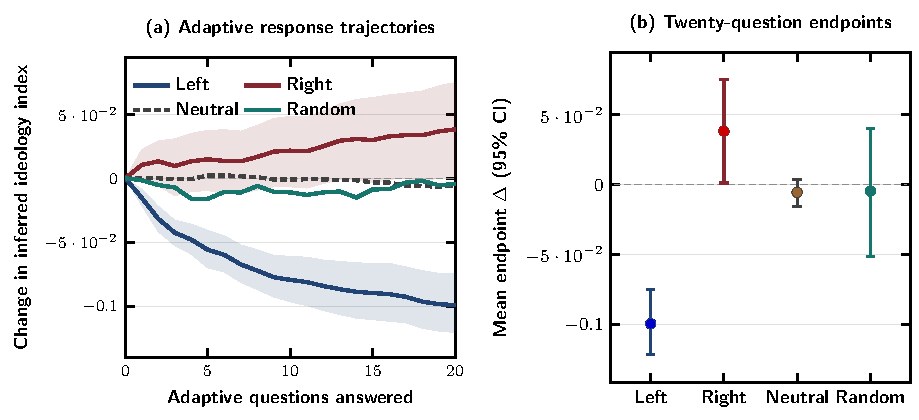
\includegraphics[width=\textwidth]{Figures/External/humanstudy}

\vspace{-10pt}
\caption{\textbf{Human study response trajectories and endpoints.}
(a) The mean change from baseline in the LSM-derived ideology coordinate as
adaptive questions are answered, with pointwise 95\% participant-bootstrap
confidence intervals shaded only for Left and Right. Partial sessions contribute
only through their last observed step. (b) Endpoint means and 95\% bootstrap
confidence intervals for all four policies, calculated from participants with
all 20 adaptive answers. Arm sample sizes are reported in
Table~\ref{tab:humanstudy-participants}.}
\label{fig:humanstudy-trajectory-endpoints}


\end{figure*}



\subsection{Interpretation}
The human results support the directional-steering hypothesis. At
question 20, Left moved the inferred ideology index by $-0.0783$
(95\% bootstrap CI $[-0.1130,-0.0195]$), and Right moved it by
$+0.0382$ (CI $[+0.0012,+0.0748]$). Neutral ($-0.0054$) and
Random ($-0.0045$) showed substantially smaller mean changes.
The Right arm included 11 participants with negative and six with
positive baseline indices; rightward mean movement therefore occurred
in a cohort spanning both sides of the initial ideology coordinate.

Together with the native simulations, these human-response results
demonstrate directional control over the \emph{inferred ideology
index} through adaptive question selection. Defining displacement
relative to each participant's own baseline allows this effect to
be evaluated across heterogeneous starting states.



\section{Discussion and Conclusion}
DTAG uses high-dimensional survey dependencies to select questions that systematically refine a predictive phenotype. The native experiments show directional movement using exclusively non-pole items; fixed-set replays indicate that selected question identities, rather than their precise order, account for much of the directionality. The index depends on the reference poles, candidate pool, and conditional model and should be interpreted as predictive position rather than a self-reported ideology score.

The human-response study confirms that adaptive questioning can steer the inferred ideology index: left- and right-directed policies yielded signed mean shifts in the intended directions, while neutral and random policies remained near zero. These movements were measured relative to each participant's starting index, including a right-policy cohort with both negative and positive baseline values.

\section*{Acknowledgments}
This work was supported by the Defense Advanced Research Projects Agency (DARPA) under the MAGICS program (DARPA-EA-25-02-05-MAGICS-PA-025; Award No.~HR0011-26-3-E016).

\bibliographystyle{IEEEtran}
\bibliography{references}

% The 10-question supplementary reversal plot is intentionally omitted.
% Its original data belong to a different experiment.
\end{document}
